% !TEX program = xelatex
\documentclass[12pt,a4paper,fontset=fandol]{ctexart}
\usepackage[left=22mm,right=22mm,top=22mm,bottom=22mm]{geometry}
\usepackage{amsmath,amssymb,bm,mathtools}
\usepackage{graphicx,xcolor,booktabs,longtable,array,calc}
\usepackage{tikz}
\usetikzlibrary{arrows.meta,calc,decorations.pathmorphing}
\usepackage{setspace,enumitem,fancyhdr}
\usepackage[unicode,hidelinks]{hyperref}
\setstretch{1.24}
\setlength{\parindent}{2em}
\setlength{\parskip}{.35em}
\setlength{\emergencystretch}{2em}
\setlist{nosep,leftmargin=2em}
\setcounter{secnumdepth}{-1}
\ctexset{section={format=\Large\bfseries,beforeskip=1em,afterskip=.7em},
subsection={format=\large\bfseries,beforeskip=.8em,afterskip=.4em},
subsubsection={format=\normalsize\bfseries,beforeskip=.7em,afterskip=.3em}}
\allowdisplaybreaks[2]
\tikzset{arr/.style={-{Stealth[length=2mm]},semithick},
dot/.style={circle,fill,inner sep=1.5pt}}
\providecommand{\tightlist}{\setlength{\itemsep}{0pt}\setlength{\parskip}{0pt}}
\providecommand{\pandocbounded}[1]{#1}
\newsavebox{\diagrambox}
\pagestyle{fancy}
\fancyhf{}
\renewcommand{\headrulewidth}{0pt}
\fancyfoot[C]{\small \thepage}
\setlength{\headheight}{16pt}
\begin{document}
\begin{titlepage}
\thispagestyle{empty}
\vspace*{27mm}
\begin{center}
{\LARGE\bfseries 第35届全国中学生物理竞赛\par}
\vspace{8mm}
{\LARGE\bfseries 复赛理论试题\par}
\vspace{17mm}
{\Large 学生详解版\par}
\end{center}
\vfill
\end{titlepage}
\setcounter{page}{1}
\section{第 1 题
地球引力场中的轨道与落地时间（40分）}\label{ux7b2c-1-ux9898-ux5730ux7403ux5f15ux529bux573aux4e2dux7684ux8f68ux9053ux4e0eux843dux5730ux65f6ux95f440ux5206}

假设地球是质量分布各向同性的球体。在离地面高度为 \(h\)
的空间站发射一个小物体，其相对于地球的初速度垂直于它到地心的连线。地球半径为
\(R\)，质量为 \(M\)，引力常量为 \(G\)。忽略地球自转及大气影响。

（1）若物体能绕地球做周期运动，其初速度大小应满足什么条件？

（2）若初速度大小为
\(v_0\)，且物体能落到地面，求落地速度的大小、速度与水平分量的夹角，以及从发射到第一次落地的时间。

已知当 \(c<0\)、\(\Delta=b^2-4ac>0\) 时，

\[
\int\frac{x\,dx}{\sqrt{a+bx+cx^2}}
=\frac{\sqrt{a+bx+cx^2}}{c}
-\frac{b}{2(-c)^{3/2}}\arcsin\frac{2cx+b}{\sqrt\Delta}+C.
\]

\begin{center}
\begin{minipage}{\linewidth}
\centering\begingroup\sbox{\diagrambox}{\small
\begin{tikzpicture}[scale=.85]
\fill[blue!10] (0,0) circle(1.5); \draw[thick] (0,0) circle(1.5);
\draw[thick,blue] (.8,0) ellipse(2.3 and 2.156);
\fill (0,0) circle(2pt) node[below] {$O$};
\fill (3.1,0) circle(2pt) node[right] {$P:r_0=R+h$};
\draw[arr,red] (3.1,0)--(3.1,1.4) node[right] {$v_0$};
\draw[dashed] (0,0)--(3.1,0); \draw[arr] (0,0)--(-1.5,0) node[midway,above] {$R$};
\node[left] at(-1.7,0) {$r_{\rm p}$};
\node at(.8,-2.65) {临界椭圆与地表相切；焦点在地心};
\end{tikzpicture}
}
\ifdim\wd\diagrambox>.88\linewidth
\sbox{\diagrambox}{\resizebox{.88\linewidth}{!}{\usebox{\diagrambox}}}\fi
\ifdim\ht\diagrambox>.38\textheight
\resizebox{!}{.38\textheight}{\usebox{\diagrambox}}
\else\usebox{\diagrambox}\fi
\par\smallskip{\small 轨道、发射点及地球表面\par}\endgroup\end{minipage}\end{center}

\subsection{一、题型定位}\label{ux4e00ux9898ux578bux5b9aux4f4d}

中心力轨道中，能量决定是否有界，角动量决定能否接近地表，时间则必须由运动方程或开普勒方程求出。只有``总能量为负''还不足以保证物体长期绕地球运行；一条有界椭圆也可能穿过地球。

发射方向是切向，所以初始径向速度为零。发射点必是一个径向转折点，但它可能是远地点，也可能是近地点。求轨道前应先确定发射点是远地点还是近地点，以免混用两个分支的条件。

\subsection{二、知识点}\label{ux4e8cux77e5ux8bc6ux70b9}

球对称引力场在地球外与地心质点等效。以下记

\[
\mu_g=GM,\qquad r_0=R+h,\qquad
\varepsilon=\frac{v_0^2}{2}-\frac{\mu_g}{r_0},
\qquad j=r_0v_0.
\]

\(\varepsilon\) 是单位质量的机械能，\(j\)
是单位质量的角动量。它们分别具有速度平方和面积除以时间的量纲。用比能、比角动量可消去小物体质量，不必在每一步重复写质量因子。

极坐标中的切向速度和径向能量关系为

\[
v_\theta=\frac{j}{r},\qquad
\frac{\dot r^2}{2}+\frac{j^2}{2r^2}-\frac{\mu_g}{r}
=\varepsilon.
\]

把后两项看作有效势，就能直接读出允许运动区间。圆轨道速度、逃逸速度分别为

\[
v_{\rm c}=\sqrt{\frac{\mu_g}{r_0}},\qquad
v_{\rm esc}=\sqrt{\frac{2\mu_g}{r_0}}.
\]

二者不是同一阈值。圆轨道速度用于区分发射点的远近地点身份，逃逸速度用于区分有界与无界运动。

\subsection{三、物理图像}\label{ux4e09ux7269ux7406ux56feux50cf}

若
\(v_0<v_{\rm c}\)，引力大于保持当前半径圆周运动所需的力，物体开始向内运动，发射点是远地点。它可能在到达近地点前先撞上地球。

若 \(v_0=v_{\rm c}\)，轨道是半径 \(r_0\) 的圆。若
\(v_{\rm c}<v_0<v_{\rm esc}\)，发射点是近地点，整个轨道的半径均不小于
\(r_0>R\)，不会撞地。

\begin{center}
\begin{minipage}{\linewidth}
\centering\begingroup\sbox{\diagrambox}{\small
\begin{tikzpicture}[xscale=1.15,yscale=1.7]
\draw[arr] (.5,-1.1)--(6.5,-1.1) node[right] {$r$};
\draw[arr] (.7,-1.2)--(.7,1.2) node[above] {$U_{\rm eff}/m$};
\draw[blue,thick,domain=.75:6,samples=100] plot(\x,{1.5/(\x*\x)-2/\x});
\draw[red] (.8,-.4)--(6,-.4) node[right] {$\varepsilon$};
\draw[dashed] (1.2,-1.05)--(1.2,.25) node[above] {$R$};
\draw[dashed] (4.08,-1.05)--(4.08,-.4) node[above] {$r_0$};
\node at(3.8,.8) {$U_{\rm eff}/m=j^2/(2r^2)-GM/r$};
\end{tikzpicture}
}
\ifdim\wd\diagrambox>.88\linewidth
\sbox{\diagrambox}{\resizebox{.88\linewidth}{!}{\usebox{\diagrambox}}}\fi
\ifdim\ht\diagrambox>.38\textheight
\resizebox{!}{.38\textheight}{\usebox{\diagrambox}}
\else\usebox{\diagrambox}\fi
\par\smallskip{\small 有效势与地表截断\par}\endgroup\end{minipage}\end{center}

图中的能量水平线与有效势相交处是径向转折点；地表不是势能曲线上的特殊点，而是题目规定的物理边界。落地时应在
\(r=R\) 截断运动，不能继续把数学椭圆的地下部分当作自由飞行。

临界椭圆恰好以地表为近地点。它给出周期轨道的下限速度，也给出落地问题中``刚好擦到地表''的极限。题目说能绕地球持续运行，按不接触地表理解时，下限必须取严格不等号。

\subsection{四、解题入口}\label{ux56dbux89e3ux9898ux5165ux53e3}

先用 \(\varepsilon<0\) 求上限，再把临界轨道的两个转折点 \(R,r_0\)
代入能量与角动量守恒求下限。这比先写出完整椭圆方程更省计算。

第二问先求速度大小，再求切向分量；径向分量由勾股关系得到，符号由``第一次向内到达地面''决定。时间不由平均速度求，而由径向速度积分求。

时间表达式可使用题给积分，也可使用偏近点角。前者直接对应守恒方程，后者让擦地极限和径向自由落体极限更容易检验。以下把两条路线都写出，以便互相检查。

\subsection{五、解析}\label{ux4e94ux89e3ux6790}

\subsubsection{1.
有界条件与临界近地点}\label{ux6709ux754cux6761ux4ef6ux4e0eux4e34ux754cux8fd1ux5730ux70b9}

有界的开普勒轨道要求

\[
\varepsilon<0
\quad\Longrightarrow\quad
v_0<\sqrt{\frac{2\mu_g}{r_0}}.
\]

在恰好擦到地表的临界轨道中，地表处的径向速度也为零。设此时发射速度为
\(v_{\min}\)、地表切向速度为 \(v_{\rm p}\)。角动量守恒给出

\[
r_0v_{\min}=Rv_{\rm p}.
\]

能量守恒给出

\[
\frac{v_{\min}^2}{2}-\frac{\mu_g}{r_0}
=\frac{v_{\rm p}^2}{2}-\frac{\mu_g}{R}.
\]

代入 \(v_{\rm p}=r_0v_{\min}/R\)，整理得到

\[
v_{\min}^2=\frac{2\mu_g R}{r_0(r_0+R)}.
\]

因此持续运行且不接触地面的答案为

\[
\boxed{\sqrt{\frac{2GMR}{(R+h)(2R+h)}}<v_0
<\sqrt{\frac{2GM}{R+h}}}.
\]

若只把``绕地球周期运动''理解为数学质点在地表无碰撞地擦过，可把左端等号单独讨论；实际地表存在接触，下限不应直接并入安全轨道范围。

\subsubsection{2.
为什么没有遗漏高速椭圆分支}\label{ux4e3aux4ec0ux4e48ux6ca1ux6709ux9057ux6f0fux9ad8ux901fux692dux5706ux5206ux652f}

两个径向转折点满足

\[
2\varepsilon r^2+2\mu_g r-j^2=0.
\]

其中一个根是 \(r_0\)。另一个根记为 \(r_*\)，由根的乘积得

\[
r_*=\frac{r_0^2v_0^2}{2\mu_g-r_0v_0^2}.
\]

当 \(v_0<v_{\rm c}\)，有 \(r_*<r_0\)，它是近地点；此时 \(r_*>R\)
正好等价于 \(v_0>v_{\min}\)。当 \(v_0>v_{\rm c}\)，有
\(r_*>r_0\)，近地点是发射点本身，已经大于 \(R\)。

所以用临界近地点求出的下限，与负能量求出的上限可以合并成一个区间。若把
\(r_*\) 一律称为近地点，则会在高速椭圆分支上错误地交换远近地点。

\subsubsection{3.
落地速度及方向}\label{ux843dux5730ux901fux5ea6ux53caux65b9ux5411}

能第一次到达地表的速度范围为
\(0\le v_0\le v_{\min}\)；等号表示擦地极限。由能量守恒，

\[
\boxed{v_R=\sqrt{v_0^2+
2\mu_g\left(\frac1R-\frac1{r_0}\right)}}.
\]

由角动量守恒，

\[
v_{\theta R}=\frac{r_0v_0}{R}.
\]

径向分量为

\[
v_{rR}=-\sqrt{v_R^2-v_{\theta R}^2}.
\]

负号表示径向向内。设速度与沿原运动方向的水平分量夹角为 \(\alpha\)，则

\[
\boxed{\alpha=\arccos\frac{r_0v_0}{Rv_R}},
\qquad 0\le\alpha\le\frac\pi2.
\]

方向可以完整表述为``沿原切向方向并向地心下倾 \(\alpha\)''。在 \(v_0=0\)
时水平分量为零，取径向落地的极限 \(\alpha=\pi/2\)；在 \(v_0=v_{\min}\)
时径向分量为零，\(\alpha=0\)。

根号是否非负也是落地条件的独立检验：

\[
v_R^2-v_{\theta R}^2
=\frac{h}{R^2r_0}
\left[2\mu_g R-v_0^2r_0(R+r_0)\right]\ge0.
\]

\subsubsection{4.
径向积分求时间}\label{ux5f84ux5411ux79efux5206ux6c42ux65f6ux95f4}

由守恒方程消去角速度，

\[
\dot r=-\sqrt{v_0^2-\frac{2\mu_g}{r_0}
+\frac{2\mu_g}{r}-\frac{j^2}{r^2}}.
\]

于是

\[
t_R=\int_R^{r_0}
\frac{r\,dr}{\sqrt{cr^2+br+a}},
\]

其中

\[
a=-j^2,\qquad b=2\mu_g,\qquad
c=v_0^2-\frac{2\mu_g}{r_0}<0.
\]

积分上端 \(r_0\) 是转折点，分母趋于零，但奇性是 \(1/\sqrt{r_0-r}\)
型，积分有限。不能因为起点径向速度为零就说落地时间无穷大。

此时

\[
\Delta=4(\mu_g-r_0v_0^2)^2>0.
\]

落地分支有 \(v_0<v_{\rm c}\)，故

\[
\frac{2cr_0+b}{\sqrt\Delta}=-1.
\]

将题给原函数在上下限作差，得较紧凑的时间表达式

\[
\boxed{
t_R=\frac{\sqrt{cR^2+bR+a}}{-c}
+\frac{b}{2(-c)^{3/2}}
\left[\frac\pi2+
\arcsin\frac{2cR+b}{\sqrt\Delta}\right]}.
\]

这里的 \(a,b,c\) 仅为积分系数，不能把 \(a\)
与下面的椭圆半长轴混用。第一项和第二项均具有时间量纲；上端根号为零已经用掉。

\subsubsection{5.
偏近点角的等价表达}\label{ux504fux8fd1ux70b9ux89d2ux7684ux7b49ux4ef7ux8868ux8fbe}

定义半长轴、偏心率与平均角速度

\[
a_{\rm K}=\frac{\mu_g}{2\mu_g/r_0-v_0^2},
\qquad e=1-\frac{r_0v_0^2}{\mu_g},
\qquad n_{\rm K}=\sqrt{\frac{\mu_g}{a_{\rm K}^3}}.
\]

本分支 \(r_0=a_{\rm K}(1+e)\)，所以发射点对应偏近点角 \(E=\pi\)。设

\[
E_R=\arccos\frac{1-R/a_{\rm K}}e,\qquad 0\le E_R\le\pi.
\]

\begin{center}
\begin{minipage}{\linewidth}
\centering\begingroup\sbox{\diagrambox}{\small
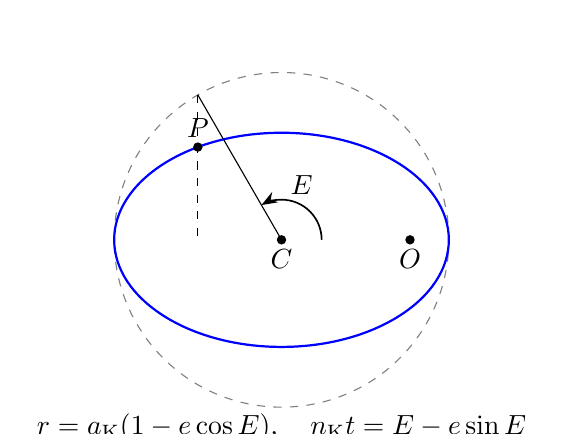
\begin{tikzpicture}[scale=.85]
\draw[gray,dashed] (0,0) circle(2.5); \draw[blue,thick] (0,0) ellipse(2.5 and 1.6);
\fill (0,0) circle(2pt) node[below] {$C$};\fill(1.92,0) circle(2pt) node[below] {$O$};
\coordinate(P) at(-1.25,1.386); \fill(P) circle(2pt) node[above] {$P$};
\draw (0,0)--(-1.25,2.165); \draw[dashed] (-1.25,2.165)--(-1.25,0);
\draw[arr] (.6,0) arc(0:120:.6) node[midway,above] {$E$};
\node at(0,-2.8) {$r=a_{\rm K}(1-e\cos E),\quad n_{\rm K}t=E-e\sin E$};
\end{tikzpicture}
}
\ifdim\wd\diagrambox>.88\linewidth
\sbox{\diagrambox}{\resizebox{.88\linewidth}{!}{\usebox{\diagrambox}}}\fi
\ifdim\ht\diagrambox>.38\textheight
\resizebox{!}{.38\textheight}{\usebox{\diagrambox}}
\else\usebox{\diagrambox}\fi
\par\smallskip{\small 偏近点角与椭圆半长轴\par}\endgroup\end{minipage}\end{center}

向内运行到地表时，连续增大的角变量是 \(E=2\pi-E_R\)。由开普勒时间方程
\(n_{\rm K}t=E-e\sin E\) 的差值，

\[
\boxed{t_R=\frac{\pi-E_R+e\sin E_R}{n_{\rm K}}}.
\]

若直接把 \(E_R-\pi\)
当作角度变化，会得到负时间；错误来自选用了椭圆另一侧的角度分支，而非守恒定律失效。

\subsubsection{6.
三个极限检查}\label{ux4e09ux4e2aux6781ux9650ux68c0ux67e5}

擦地时 \(R=a_{\rm K}(1-e)\)，故 \(E_R=0\)。落地时间等于半周期：

\[
t_R=\pi\sqrt{\frac{[(r_0+R)/2]^3}{\mu_g}}.
\]

径向释放 \(v_0=0\)
时，\(a_{\rm K}=r_0/2,e=1\)，可将椭圆表达式视为退化极限，得到

\[
t_R=\sqrt{\frac{r_0^3}{2\mu_g}}
\left[\arccos\sqrt{\frac R{r_0}}
+\sqrt{\frac R{r_0}\left(1-\frac R{r_0}\right)}\right].
\]

最后，当 \(h\ll R\) 且 \(v_0=0\)，地表重力近似
\(g_R=\mu_g/R^2\)，展开上式有

\[
t_R\simeq\sqrt{\frac{2h}{g_R}}.
\]

三个检查分别检验椭圆时间尺度、零角动量分支和近地匀加速近似；它们检验的是不同环节，不能只用一个量纲检查代替。

\par\noindent\begin{minipage}{\linewidth}
\subsubsection{7.
无量纲化后的具体算例}\label{ux65e0ux91cfux7eb2ux5316ux540eux7684ux5177ux4f53ux7b97ux4f8b}

为看清各式的尺度，取长度单位为 \(R\)，速度单位为
\(\sqrt{\mu_g/R}\)，时间单位为 \(\sqrt{R^3/\mu_g}\)。令发射半径为
\(r_0=2R\)，无量纲初速度为 \(0.3\)。

圆轨道速度为 \(1/\sqrt2\)，擦地速度为 \(1/\sqrt3\)。由于
\(0.3<1/\sqrt3\)，本例确实落地。无量纲落地速度及切向分量为

\[
\widehat v_R=\sqrt{1.09},\qquad
\widehat v_{\theta R}=0.6.
\]

因此

\[
\cos\alpha=\frac{0.6}{\sqrt{1.09}},
\qquad
\widehat v_{rR}=-\sqrt{1.09-0.36}.
\]

半长轴和偏心率为

\[
\widehat a_{\rm K}=\frac1{1-0.3^2},
\qquad e=1-2(0.3)^2=0.82.
\]

把它们代入偏近点角时间式，可与直接积分径向速度或二维牛顿方程比较。这个算例不使用地球实际数值，仍能检查转折点、分支和单位尺度。

若换回任意地球模型，只需分别乘对应的速度和时间单位。无量纲化还避免把很大的地心距离与很小的积分误差混在一起，是计算核验中心力轨道的实用方法。

\end{minipage}\par
\clearpage

\section{第 2 题
干摩擦弹簧振子的有限次往返（40分）}\label{ux7b2c-2-ux9898-ux5e72ux6469ux64e6ux5f39ux7c27ux632fux5b50ux7684ux6709ux9650ux6b21ux5f80ux8fd440ux5206}

轻弹簧左端固定，右端连接质量为 \(m\) 的小球，劲度系数为
\(k\)。弹簧水平，自然长度位置为坐标原点
\(O\)。小球在水平地面上滑动，动摩擦因数为 \(\mu\)，重力加速度为
\(g\)；最大静摩擦力等于滑动摩擦力。初始速度为零，初始伸长为
\(-A_0\)，其中 \(A_0>0\)，但 \(A_0\) 不是已知量。

（1）如果小球至多只能向右运动，求最终静止位置，以及 \(A_0\)
应满足的条件。

（2）如果小球完成第一次向右运动至原点右边后，至多只能向左运动，求最终静止位置，以及
\(A_0\) 应满足的条件。

（3）如果小球只能完成 \(n\) 次往返运动，求最终静止位置，以及 \(A_0\)
应满足的条件。向右经过原点，然后向左经过原点，算一次往返。

（4）如果小球只能完成 \(n\) 次往返运动，求从开始运动至最终静止的总路程。

\begin{center}
\begin{minipage}{\linewidth}
\centering\begingroup\sbox{\diagrambox}{\small
\begin{tikzpicture}[scale=.9]
\draw[thick](-4,-.3)--(4,-.3); \draw[thick](-4,-.3)--(-4,1.1);
\draw[decorate,decoration={coil,aspect=.4,segment length=4pt,amplitude=4pt}](-4,.3)--(-1.8,.3);
\draw[thick,fill=gray!15](-1.8,0)rectangle(-1.2,.6); \node at(-1.5,.3){$m$};
\draw[arr](-4,-.8)--(4.5,-.8)node[right]{$x$};
\draw[dashed](0,-1)--(0,1)node[above]{$O$};\node[below]at(-1.5,-.8){$-A_0$};
\draw[arr,red](-1.2,.6)--(.2,.6)node[above]{$kx$的回复方向};
\draw[arr,blue](-1.8,0)--(-3,0)node[below]{$f=\mu mg$};
\end{tikzpicture}
}
\ifdim\wd\diagrambox>.88\linewidth
\sbox{\diagrambox}{\resizebox{.88\linewidth}{!}{\usebox{\diagrambox}}}\fi
\ifdim\ht\diagrambox>.38\textheight
\resizebox{!}{.38\textheight}{\usebox{\diagrambox}}
\else\usebox{\diagrambox}\fi
\par\smallskip{\small 初始压缩、坐标与右行时的摩擦力\par}\endgroup\end{minipage}\end{center}

\subsection{一、题型定位}\label{ux4e00ux9898ux578bux5b9aux4f4d-1}

本题应按摩擦方向分段求解，并在每个转折点判断小球能否继续运动；振幅不按指数规律衰减。滑动时摩擦力大小固定、方向随速度反向；静止时摩擦力自动调整，只有超过最大静摩擦力才能重新启动。

题目对一次往返的定义特别重要：必须向右、向左都经过原点。发生一次速度反向不必然等于完成半次往返；最后一段运动还可能完全位于原点同一侧。

\subsection{二、知识点}\label{ux4e8cux77e5ux8bc6ux70b9-1}

记

\[
f=\mu mg,\qquad b=\frac fk,\qquad
\omega=\sqrt{\frac km}.
\]

\(b\) 是静摩擦能平衡弹簧力的最大位移。因此速度为零时，

\[
|x|\le b\quad\Longrightarrow\quad\text{可以保持静止}.
\]

若
\(|x|>b\)，小球必然向原点方向重新启动。等号处能够静止，题给初始静止状态不应凭空启动。

滑动时的方程分别为

\[
\ddot x+\omega^2(x+b)=0\quad(\dot x>0),
\]

\[
\ddot x+\omega^2(x-b)=0\quad(\dot x<0).
\]

所以每一单向滑动段都相当于围绕一个偏移平衡位置作半个简谐周期；右行的中心在
\(-b\)，左行的中心在 \(b\)。

\subsection{三、物理图像}\label{ux4e09ux7269ux7406ux56feux50cf-1}

\begin{center}
\begin{minipage}{\linewidth}
\centering\begingroup\sbox{\diagrambox}{\small
\begin{tikzpicture}[scale=.85]
\draw[arr](-5,0)--(5,0)node[right]{$x$};
\fill[green!15](-.7,-.3)rectangle(.7,.3);
\node[below]at(-.7,-.3){$-b$};\node[below]at(.7,-.3){$b$};
\foreach \x/\s in {-4/A_0,2.6/A_0-2b,-1.2/4b-A_0}{\fill(\x,0)circle(2pt);}
\draw[arr,blue](-4,.8)--(2.6,.8)node[midway,above]{右行：$x_1=-2b-x_0$};
\draw[arr,red](2.6,1.7)--(-1.2,1.7)node[midway,above]{左行：$x_2=2b-x_1$};
\node at(0,-1.1){停在静摩擦带内时，不能直接续用转折点递推};
\end{tikzpicture}
}
\ifdim\wd\diagrambox>.88\linewidth
\sbox{\diagrambox}{\resizebox{.88\linewidth}{!}{\usebox{\diagrambox}}}\fi
\ifdim\ht\diagrambox>.38\textheight
\resizebox{!}{.38\textheight}{\usebox{\diagrambox}}
\else\usebox{\diagrambox}\fi
\par\smallskip{\small 转折点递推和静摩擦带\par}\endgroup\end{minipage}\end{center}

图中的绿色区间 \([-b,b]\)
是停止带。小球到达速度为零的位置后，先看是否落入这一区间，再决定能否进入下一段。不能为了保持递推形式而人为添加已经不存在的运动段。

若从很大的负位移释放，第一次右端转折点大约比初始振幅小
\(2b\)；再回到左端，振幅又小 \(2b\)。每个真正的完整往返降低幅度 \(4b\)。

\begin{center}
\begin{minipage}{\linewidth}
\centering\begingroup\sbox{\diagrambox}{\small
\begin{tikzpicture}[xscale=1.1,yscale=.85]
\draw[arr](0,0)--(8,0)node[right]{$A_0/b$};
\draw[arr](0,-1.4)--(0,1.8)node[above]{$x_f/b$};
\draw[blue,thick](0,0)--(1,-1)--(3,1)--(5,-1)--(7,1);
\draw[dashed](0,1)--(7.4,1);\draw[dashed](0,-1)--(7.4,-1);
\foreach \x in {1,3,5,7}{\draw[dashed](\x,-1.1)--(\x,1.2);\node[below]at(\x,-1.2){$\x$};}
\node at(4,2){终点在$[-b,b]$内呈折线变化};
\end{tikzpicture}
}
\ifdim\wd\diagrambox>.88\linewidth
\sbox{\diagrambox}{\resizebox{.88\linewidth}{!}{\usebox{\diagrambox}}}\fi
\ifdim\ht\diagrambox>.38\textheight
\resizebox{!}{.38\textheight}{\usebox{\diagrambox}}
\else\usebox{\diagrambox}\fi
\par\smallskip{\small 最终位置随初始压缩量变化\par}\endgroup\end{minipage}\end{center}

最终位置并不总在左边，也不总等于零。图中的折线说明：连续改变初始压缩量，最后一段可能右行或左行，终点在停止带内来回移动。这种终点结构来自静摩擦，不是最后一次振幅必须恰好耗尽。

\subsection{四、解题入口}\label{ux56dbux89e3ux9898ux5165ux53e3-1}

第一步只研究``从某个静止端点出发，到下一次速度为零''的单段映射。第二步把每个端点与
\(b\) 比较。第三步根据题目对往返的定义，用过零次数而非转向次数计数。

求总路程可直接计算整个过程的能量耗散。由于每一段摩擦耗散均为 \(f\)
乘路程，得到终点后即可求总路程，无须把很多段距离逐个相加。

以下默认 \(\mu>0\)。若
\(\mu=0\)，停止带缩成一个点，小球无耗散地振动，题目所说最终停止的情形不成立，不能把含
\(1/\mu\) 的公式直接代入。

\subsection{五、解析}\label{ux4e94ux89e3ux6790-1}

\subsubsection{1.
单段运动及端点映射}\label{ux5355ux6bb5ux8fd0ux52a8ux53caux7aefux70b9ux6620ux5c04}

从 \(x_i<-b\) 静止启动向右，解动力学方程得

\[
x(t)=-b+(x_i+b)\cos\omega t.
\]

第一次再次速度为零发生在 \(\omega t=\pi\)，此时

\[
x_{i+1}=-2b-x_i.
\]

特别地，从 \(x_0=-A_0\) 出发，

\[
x_1=A_0-2b.
\]

也可由动能定理独立推导：

\[
\frac k2(A_0^2-x_1^2)=f(A_0+x_1).
\]

消去非零路程因子 \(A_0+x_1\)，同样得到 \(x_1=A_0-2b\)。只有 \(A_0>b\)
时小球才会滑动，故不能把这个映射用于 \(A_0\le b\) 的初始静止状态。

从 \(x_i>b\) 静止启动向左时，同理

\[
x(t)=b+(x_i-b)\cos\omega t,\qquad
x_{i+1}=2b-x_i.
\]

两条映射的常数项符号相反，反映摩擦力方向的改变。

\subsubsection{2.
第一问：至多向右运动}\label{ux7b2cux4e00ux95eeux81f3ux591aux5411ux53f3ux8fd0ux52a8}

若 \(0<A_0\le b\)，弹簧力没有超过最大静摩擦力，小球完全不动：

\[
\boxed{x_f=-A_0,\quad 0<A_0\le b}.
\]

若 \(A_0>b\)，第一段右行的终点为 \(x_1=A_0-2b\)。要在那里停住，必须
\(|x_1|\le b\)，即

\[
b<A_0\le3b.
\]

因此另一个分支为

\[
\boxed{x_f=A_0-2b,\quad b<A_0\le3b}.
\]

在 \(b<A_0\le2b\) 时，小球最终停在原点左侧或原点；在 \(2b<A_0\le3b\)
时，它向右过原点后停在右侧。只有
\(A_0>3b\)，才有足够的回复力开始向左运动。

\subsubsection{3.
第二问：第一段过零后至多左行}\label{ux7b2cux4e8cux95eeux7b2cux4e00ux6bb5ux8fc7ux96f6ux540eux81f3ux591aux5de6ux884c}

把第一段确实向右经过原点写成 \(A_0>2b\)。若
\(2b<A_0\le3b\)，到右端后直接静止，这已包含在第一问。题目使用``至多''，从字面上说该重叠分支也符合第二问。

参考解答主要讨论第一段之后确实开始向左的新增情形：\(A_0>3b\)。左行终点为

\[
x_2=2b-x_1=4b-A_0.
\]

要求左行后不再右行，即 \(|x_2|\le b\)，得到

\[
\boxed{x_f=4b-A_0,\quad3b<A_0\le5b}.
\]

其中 \(3b<A_0<4b\)
时，左行到原点右边便停住，未完成题定义的一次往返；\(A_0=4b\)
时恰好停在原点，也没有向左经过原点。只有 \(4b<A_0\le5b\)
才完成了一次往返。

明确这一区别之后，后面的计数就不容易在 \(A_0=4nb\) 处错一个单位。

\subsubsection{4.
多段递推与往返次数}\label{ux591aux6bb5ux9012ux63a8ux4e0eux5f80ux8fd4ux6b21ux6570}

只要各中间端点仍能启动，端点公式可统一写成

\[
x_j=(-1)^{j+1}(A_0-2jb),\qquad j=0,1,2,\ldots.
\]

这里 \(j=0\) 也正确给出
\(x_0=-A_0\)。对于前面真实存在的往返，偶数端点在左侧，奇数端点在右侧。

完成第 \(n\) 次向左过原点，需要

\[
x_{2n}=4nb-A_0<0
\quad\Longrightarrow\quad A_0>4nb.
\]

不能完成第 \(n+1\) 次往返，需要

\[
A_0\le4(n+1)b.
\]

因此对 \(n\ge1\)，恰好完成 \(n\) 次往返的总范围是

\[
\boxed{4nb<A_0\le4(n+1)b}.
\]

左端严格，是因为``停在原点''不等于``经过原点''。右端包含，是因为下一次向左运动恰好到原点便停。

\subsubsection{5.
第三问的终点分段}\label{ux7b2cux4e09ux95eeux7684ux7ec8ux70b9ux5206ux6bb5}

在上述总范围内，有三种停止方式。若

\[
4nb<A_0\le(4n+1)b,
\]

小球在完成第 \(n\) 次往返的左端直接停住：

\[
\boxed{x_f=4nb-A_0}.
\]

若

\[
(4n+1)b<A_0\le(4n+3)b,
\]

它又开始右行，然后停住，终点为

\[
\boxed{x_f=A_0-(4n+2)b}.
\]

这个区间可在 \((4n+2)b\)
处分成两段：前半终点在左侧，后半在右侧，但表达式相同，可以合并书写。

若

\[
(4n+3)b<A_0\le(4n+4)b,
\]

它再开始左行，却不能向左经过原点，终点为

\[
\boxed{x_f=(4n+4)b-A_0}.
\]

三个分支在连接处连续，且均满足
\(|x_f|\le b\)。参考解答把中间区间拆为两个符号分支；合并并不删去任何运动情形。

\subsubsection{6.
第四问：总路程}\label{ux7b2cux56dbux95eeux603bux8defux7a0b}

初态和末态动能都为零，弹簧弹性势能的减少全部变成摩擦耗散：

\[
\frac{kA_0^2}{2}-\frac{kx_f^2}{2}=fs.
\]

所以统一表达式是

\[
\boxed{s=\frac{A_0^2-x_f^2}{2b}}.
\]

代入第三问的三段终点，

\[
s=
\begin{cases}
4n(A_0-2nb),&
4nb<A_0\le(4n+1)b,\\
(4n+2)\bigl[A_0-(2n+1)b\bigr],&
(4n+1)b<A_0\le(4n+3)b,\\
(4n+4)\bigl[A_0-(2n+2)b\bigr],&
(4n+3)b<A_0\le(4n+4)b.
\end{cases}
\]

中间一段也可写成
\(2(2n+1)[A_0-(2n+1)b]\)。每一式括号内都有长度量纲，前面的数值因子无量纲。

\subsubsection{7.
任意初始压缩量的简明算法}\label{ux4efbux610fux521dux59cbux538bux7f29ux91cfux7684ux7b80ux660eux7b97ux6cd5}

如果不预先给出 \(n\)，可先计算实际单向滑动段数

\[
N_s=\max\left\{0,\left\lceil\frac{A_0/b-1}{2}\right\rceil\right\}.
\]

那么

\[
x_f=(-1)^{N_s+1}(A_0-2N_sb).
\]

取整符号必须是向上取整。在恰好到达停止带边界的参数点，上一段已经停止，所以不能再加一段。该公式给出的最后端点不一定与前面端点同样交替过零。

往返次数为

\[
n_{\rm round}=\max\left\{0,\left\lceil\frac{A_0}{4b}\right\rceil-1\right\}.
\]

例如 \(A_0=4b\) 时，虽然向右和向左都运动过，但左行恰好停在原点，故
\(n_{\rm round}=0\)；稍增至 \(4b+\epsilon\) 就完成一次往返。

\subsubsection{8.
时间及整体一致性}\label{ux65f6ux95f4ux53caux6574ux4f53ux4e00ux81f4ux6027}

每个实际滑动段都持续
\(\pi/\omega\)，最后一段也是如此；停止并非滑到静摩擦带边界瞬间发生，而是在带内某处速度真正变为零时发生。因此

\[
T_{\rm stop}=N_s\frac\pi\omega.
\]

如果以``进入
\([-b,b]\)''为事件直接终止数值积分，会过早停止。该区间只给出速度为零后的静止条件，不能对运动中的小球直接使用。

把分段路程相加应与整体能量式一致。终点折线在连接处连续，总路程也连续；停止时间却可能发生一个半周期的跳变，因为临界参数两侧真实滑动段数不同。

\subsubsection{9.
过零速度与单段速度峰}\label{ux8fc7ux96f6ux901fux5ea6ux4e0eux5355ux6bb5ux901fux5ea6ux5cf0}

从 \(-A_0\) 开始右行，若能到原点，所消耗摩擦功为
\(fA_0\)。原点处的动能是

\[
\frac12mv_O^2=\frac12kA_0^2-fA_0,
\]

故

\[
v_O^2=\omega^2A_0(A_0-2b).
\]

这独立给出第一次真正过零的条件
\(A_0>2b\)。若等号，速度在原点恰好变零，只能说到达原点。若右侧为负，说明运动根本到不了原点，不能把它理解成虚数速度的物理运动。

右行过程中加速度为 \(-\omega^2(x+b)\)，所以速度峰出现在 \(x=-b\)，而非
\(x=0\)：

\[
v_{\max}=\omega(A_0-b).
\]

这是每段简谐中心偏移的另一种表现。对多段运动，只需用该段起点的位移重新列能量式，不能把第一段的
\(A_0\) 原封不动用于所有过零速度。

全程耗散占初始弹性能的比例为

\[
\eta_{\rm heat}=1-\frac{x_f^2}{A_0^2}.
\]

因为
\(|x_f|\le b\)，大幅度释放时几乎全部初始能量变为热，但最后仍可留下不为零的弹性能和位移。能量``几乎耗尽''并不等于终点``恰在原点''。

\clearpage

\section{第 3 题
打击中心、转轴反力与撤轴后的刚体运动（40分）}\label{ux7b2c-3-ux9898-ux6253ux51fbux4e2dux5fc3ux8f6cux8f74ux53cdux529bux4e0eux64a4ux8f74ux540eux7684ux521aux4f53ux8fd0ux52a840ux5206}

质量为 \(M\)、长为 \(l\) 的匀质细杆 \(AB\) 自由悬挂于过原点 \(O\)
的水平光滑转轴上。杆在竖直的 \(xy\) 平面内转动，\(x\) 轴水平向右、\(y\)
轴竖直向上；初始上端 \(A\) 与 \(O\) 重合，杆竖直下垂。\(O\)
距地面足够高。

质量为 \(m\) 的弹丸以大小为 \(v_0\)
的水平速度从右向左撞击杆的打击中心，并很快嵌入杆中。打击过程中转轴对杆的水平作用力为零。杆转半圈到竖直向上时立即撤除转轴。重力加速度为
\(g\)。

（1）求打击中心到 \(O\) 的距离。

（2）撤轴前，求杆被撞后转过
\(\theta\)（\(0\le\theta<\pi\)）时转轴对杆的作用力。

（3）以撤轴瞬间为 \(t=0\)，求撤轴后、杆着地前杆端 \(B\) 的
\(x_B(t),y_B(t)\)。

（4）求撤轴后杆再转半圈时，固定空间点 \(O\) 与杆端 \(B\) 的高度差。

\begin{center}
\begin{minipage}{\linewidth}
\centering\begingroup\sbox{\diagrambox}{\small
\begin{tikzpicture}[scale=.9]
\draw[arr](0,0)--(3.2,0)node[right]{$x$};\draw[arr](0,-3.5)--(0,1)node[above]{$y$};
\draw[very thick](0,0)--(0,-3);\node[above left]at(0,0){$O=A$};
\fill(0,-2)circle(3pt)node[left]{$D,\ OD=2l/3$};\node[left]at(0,-3){$B$};
\draw[arr,red](2,-2)--(.2,-2)node[midway,above]{$v_0$};
\fill(2,-2)circle(3pt)node[right]{$m$};\node[left]at(0,-1){$M,l$};
\end{tikzpicture}
}
\ifdim\wd\diagrambox>.88\linewidth
\sbox{\diagrambox}{\resizebox{.88\linewidth}{!}{\usebox{\diagrambox}}}\fi
\ifdim\ht\diagrambox>.38\textheight
\resizebox{!}{.38\textheight}{\usebox{\diagrambox}}
\else\usebox{\diagrambox}\fi
\par\smallskip{\small 弹丸向左撞击竖直杆及打击中心\par}\endgroup\end{minipage}\end{center}

\subsection{一、题型定位}\label{ux4e00ux9898ux578bux5b9aux4f4d-2}

运动分为非弹性碰撞、绕固定轴转动和撤轴后的自由运动三个阶段。进入下一阶段时，应重新选定研究系统，检查约束和守恒条件。

打击中心使转轴不承受水平冲量，但不意味着随后转轴没有反力。碰撞结束后重力、向心加速度和切向加速度共同决定轴反力。

\subsection{二、知识点}\label{ux4e8cux77e5ux8bc6ux70b9-2}

匀质杆对端点的转动惯量为 \(I_{\rm rod}=Ml^2/3\)。若水平冲量 \(J\)
作用于距轴 \(d\) 处，杆的角速度改变量满足

\[
I_{\rm rod}\Delta\omega=Jd.
\]

杆质心速度改变量大小是
\((l/2)\Delta\omega\)。当转轴水平冲量为零，杆的质心动量改变必须完全由
\(J\) 提供。

碰撞时通常只守恒相应的动量或角动量，不守恒机械能。碰撞后固定轴转动时，轴反力作用点不动、不做功，所以机械能守恒。撤轴后重力对组合质心的总力矩为零，组合体相对质心的角速度恒定。

\subsection{三、物理图像}\label{ux4e09ux7269ux7406ux56feux50cf-2}

取 \(\theta\)
为从竖直下垂方向开始的顺时针转角。弹丸向左撞击，使杆先向左摆，最终到达竖直向上位置。下述公式采用这一方向约定。

\begin{center}
\begin{minipage}{\linewidth}
\centering\begingroup\sbox{\diagrambox}{\small
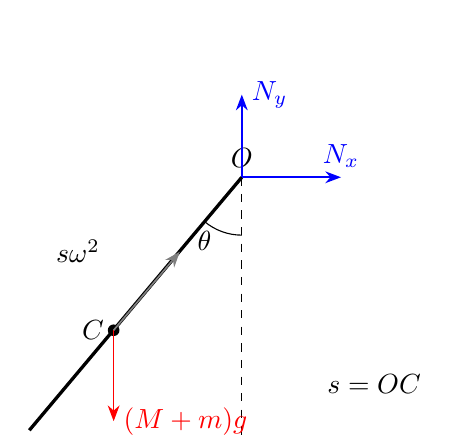
\begin{tikzpicture}[scale=1.05]
\coordinate(C)at(-1.55,-1.85); \draw[very thick](0,0)--(-2.57,-3.06);
\node[above]at(0,0){$O$};\fill(C)circle(2pt)node[left]{$C$};
\draw[dashed](0,0)--(0,-3.3);\draw (0,-.7) arc(-90:-130:.7)node[below]{$\theta$};
\draw[arr,blue](0,0)--(1.2,0)node[above]{$N_x$};
\draw[arr,blue](0,0)--(0,1)node[right]{$N_y$};
\draw[arr,red](C)--++(0,-1.1)node[right]{$(M+m)g$};
\draw[arr,gray](C)--++(.8,.95);\node[left]at(-1.6,-.9){$s\omega^2$};
\node at(1.6,-2.5){$s=OC$};
\end{tikzpicture}
}
\ifdim\wd\diagrambox>.88\linewidth
\sbox{\diagrambox}{\resizebox{.88\linewidth}{!}{\usebox{\diagrambox}}}\fi
\ifdim\ht\diagrambox>.38\textheight
\resizebox{!}{.38\textheight}{\usebox{\diagrambox}}
\else\usebox{\diagrambox}\fi
\par\smallskip{\small 组合质心、重力与转轴反力\par}\endgroup\end{minipage}\end{center}

杆和嵌入的弹丸组成刚体。其组合质心不在杆中点，而在两者质量的一阶矩平均位置。求轴反力时必须对这一组合质心应用牛顿第二定律。

\begin{center}
\begin{minipage}{\linewidth}
\centering\begingroup\sbox{\diagrambox}{\small
\begin{tikzpicture}[scale=.8]
\draw[arr](-1,0)--(7,0)node[right]{$x$};\draw[arr](0,-1)--(0,4.3)node[above]{$y$};
\draw[very thick](0,0)--(0,3.5);\fill(0,2.1)circle(2pt)node[left]{$C(0)=s$};\node[above]at(0,3.5){$B$};
\draw[arr,red](0,2.1)--(1.5,2.1)node[above]{$s\omega_*$};
\draw[blue,dashed,domain=0:5,samples=40]plot(\x,{2.1-.045351*\x*\x});
\draw[very thick](.563,1.051)--(3.825,2.319);\fill(2.52,1.812)circle(2pt)node[below right]{$C(t)$};
\draw[arr](2.8,2.8)arc(115:30:.6);
\node at(3.1,5.0){质心平抛，杆相对质心匀速转动};
\end{tikzpicture}
}
\ifdim\wd\diagrambox>.88\linewidth
\sbox{\diagrambox}{\resizebox{.88\linewidth}{!}{\usebox{\diagrambox}}}\fi
\ifdim\ht\diagrambox>.38\textheight
\resizebox{!}{.38\textheight}{\usebox{\diagrambox}}
\else\usebox{\diagrambox}\fi
\par\smallskip{\small 撤轴后质心平抛与绕质心匀速转动\par}\endgroup\end{minipage}\end{center}

撤轴瞬间，上端 \(B\)
向右运动，组合质心也向右运动。此后整个刚体的质心作平抛，杆相对质心作顺时针匀速转动。杆端轨迹是平抛和圆周运动叠加，不是一个简单抛物线。

\subsection{四、解题入口}\label{ux56dbux89e3ux9898ux5165ux53e3-2}

先用``杆的水平冲量''和``杆绕端点的角冲量''联立求打击中心。再对碰撞后的组合体计算质心距轴
\(s\) 与转动惯量 \(I_O\)，统一使用这两个参数。

轴反力可以不先求展开的复杂表达式：写出质心位置，求两次导数，再乘总质量并加重力项。用
\(\omega^2(\theta)\) 和 \(\ddot\theta\) 表示的结果更易检查符号。

撤轴前后角速度连续，但转轴反力突然消失。撤轴后的旋转中心应选组合质心，而不能继续把原点
\(O\) 当作转轴。

\subsection{五、解析}\label{ux4e94ux89e3ux6790-2}

\subsubsection{1. 打击中心}\label{ux6253ux51fbux4e2dux5fc3}

设打击点距 \(O\) 为
\(d\)。忽略碰撞过程中的重力冲量，对杆的角冲量方程给出

\[
\Delta\omega=\frac{Jd}{Ml^2/3}.
\]

杆质心向左的速度改变量为 \((l/2)\Delta\omega\)。由于转轴没有水平冲量，

\[
J=M\frac l2\Delta\omega.
\]

消去 \(J,\Delta\omega\)，得

\[
\boxed{d=\frac{2l}{3}}.
\]

这里求的是碰撞前杆的打击中心，使用的是杆本身的质心和惯量。不能先加入弹丸质量再计算一个``新的打击中心''，因为题目的冲击条件针对原来的杆。

\subsubsection{2.
碰撞后的参数与角速度}\label{ux78b0ux649eux540eux7684ux53c2ux6570ux4e0eux89d2ux901fux5ea6}

组合质量记为 \(\mathcal M=M+m\)，质心距轴为

\[
s=\frac{M(l/2)+m(2l/3)}{M+m}
=\frac{(3M+4m)l}{6(M+m)}.
\]

组合体对轴的惯量为

\[
I_O=\frac{Ml^2}{3}+m\left(\frac{2l}{3}\right)^2
=\frac{(3M+4m)l^2}{9}.
\]

碰撞期间，轴作用力对 \(O\) 的力矩为零，故角动量守恒：

\[
mv_0\frac{2l}{3}=I_O\omega_0.
\]

因此

\[
\boxed{\omega_0=\frac{6mv_0}{(3M+4m)l}}.
\]

质心速度大小为
\(s\omega_0=mv_0/(M+m)\)，与无水平外冲量时的总水平动量守恒相符。两条计算路线相互一致。

\subsubsection{3.
碰撞损失与随后能量守恒}\label{ux78b0ux649eux635fux5931ux4e0eux968fux540eux80fdux91cfux5b88ux6052}

碰撞后的转动动能为

\[
K_+=\frac12 I_O\omega_0^2
=\frac{2m^2v_0^2}{3M+4m}.
\]

与碰撞前弹丸动能比较，

\[
\frac{K_+}{K_-}=\frac{4m}{3M+4m}<1.
\]

损失为

\[
K_--K_+=\frac{3Mm v_0^2}{2(3M+4m)}.
\]

这一步明确非弹性嵌入不能使用机械能守恒。碰撞完成之后，轴不做功，才可在不同
\(\theta\) 之间使用机械能守恒。

\subsubsection{4.
固定轴阶段的角速度与角加速度}\label{ux56faux5b9aux8f74ux9636ux6bb5ux7684ux89d2ux901fux5ea6ux4e0eux89d2ux52a0ux901fux5ea6}

组合质心位置为

\[
x_C=-s\sin\theta,\qquad y_C=-s\cos\theta.
\]

从最低点升到角度 \(\theta\)，重力势能增加
\(\mathcal Mgs(1-\cos\theta)\)，所以

\[
\frac12I_O\omega_0^2
=\frac12I_O\omega^2+\mathcal Mgs(1-\cos\theta).
\]

由于 \(2\mathcal M s/I_O=3/l\)，

\[
\boxed{\omega^2(\theta)=\omega_0^2-
\frac{3g}{l}(1-\cos\theta)}.
\]

重力对轴产生反向力矩，故

\[
\boxed{\ddot\theta=-\frac{\mathcal Mgs}{I_O}\sin\theta
=-\frac{3g}{2l}\sin\theta}.
\]

这里 \(\omega=\dot\theta>0\) 是顺时针转动的大小，而 \(\ddot\theta\)
可为负。正负约定应贯穿位置、速度和力矩，不应只在最终结果前补一个符号。

\subsubsection{5. 转轴反力}\label{ux8f6cux8f74ux53cdux529b}

对质心坐标求导，

\[
\ddot x_C=s(\omega^2\sin\theta-\ddot\theta\cos\theta),
\]

\[
\ddot y_C=s(\omega^2\cos\theta+\ddot\theta\sin\theta).
\]

设轴对杆与弹丸整体的反力为
\(\mathbf N=N_x\mathbf i+N_y\mathbf j\)。牛顿第二定律给出

\[
N_x=\mathcal M\ddot x_C,\qquad
N_y-\mathcal Mg=\mathcal M\ddot y_C.
\]

于是

\[
\boxed{N_x=\mathcal Ms\left[
\omega^2+\frac{3g}{2l}\cos\theta\right]\sin\theta},
\]

\[
\boxed{N_y=\mathcal M\left[
g+s\omega^2\cos\theta-\frac{3gs}{2l}\sin^2\theta\right]}.
\]

其中 \(\omega^2\) 使用上一节表达式。若题目要求大小和方向，可继续写

\[
N=\sqrt{N_x^2+N_y^2},
\]

并用两分量的符号确定象限。给出 \(N_x,N_y\)
已完整确定矢量，且比反正切表达式更不易遗漏象限。

这里把``杆''理解为嵌入弹丸后的整体；嵌入处内力不作为额外外力加入。若单独对裸杆列方程，还需要弹丸对杆的未知接触力，计算会更繁琐。

\subsubsection{6.
端点反力与到达顶部条件}\label{ux7aefux70b9ux53cdux529bux4e0eux5230ux8fbeux9876ux90e8ux6761ux4ef6}

在最低点 \(\theta=0\)，

\[
N_x=0,\qquad N_y=\mathcal M(g+s\omega_0^2).
\]

在顶部 \(\theta=\pi\)，

\[
\omega_*^2=\omega_0^2-\frac{6g}{l},
\qquad N_x=0,\quad N_y=\mathcal M(g-s\omega_*^2).
\]

光滑转轴可以向上或向下施力，不存在绳子的``拉力必须非负''限制。不能额外要求顶部
\(N_y\ge0\)。

题设要在有限时间转到顶部并撤轴，实际隐含

\[
\omega_*^2>0,\qquad
v_0>\frac{3M+4m}{6m}\sqrt{6gl}.
\]

若恰好等号，顶部速度为零，物体只在无限时间极限接近不稳定顶部。此时不能继续使用
\(\pi/\omega_*\) 求再转半圈的时间。

\subsubsection{7.
撤轴后为何角速度不变}\label{ux64a4ux8f74ux540eux4e3aux4f55ux89d2ux901fux5ea6ux4e0dux53d8}

撤轴后唯一外力是均匀重力。重力的合力通过组合质心，故对质心的力矩为零。其质心惯量为

\[
I_C=I_O-\mathcal Ms^2
=\frac{M(3M+4m)l^2}{36(M+m)}.
\]

因此 \(I_C\omega\) 守恒，且 \(I_C\) 固定，角速度就是
\(\omega_*\)。这不是说相对于原点 \(O\) 的角动量仍守恒；均匀重力对固定点
\(O\) 一般有非零力矩。

撤轴瞬间质心在 \((0,s)\)，速度为 \((s\omega_*,0)\)。故

\[
x_C(t)=s\omega_*t,\qquad
y_C(t)=s-\frac12gt^2.
\]

\subsubsection{8.
杆端坐标与高度差}\label{ux6746ux7aefux5750ux6807ux4e0eux9ad8ux5ea6ux5dee}

撤轴瞬间 \(B\) 在质心上方，距离 \(l-s\)。顺时针转动后，相对质心坐标为

\[
x_{B/C}=(l-s)\sin\omega_*t,\qquad
y_{B/C}=(l-s)\cos\omega_*t.
\]

于是

\[
\boxed{x_B(t)=s\omega_*t+(l-s)\sin\omega_*t},
\]

\[
\boxed{y_B(t)=s-\frac12gt^2+(l-s)\cos\omega_*t}.
\]

在 \(t=0\)，两式给出 \(x_B=0,y_B=l\)；求导得到
\(\dot x_B=l\omega_*,\dot y_B=0\)，与撤轴前顶部端点速度连续。

再转半圈时 \(t_\pi=\pi/\omega_*\)，有

\[
y_B(t_\pi)=2s-l-\frac{g\pi^2}{2\omega_*^2}
=\frac{ml}{3(M+m)}-\frac{g\pi^2}{2\omega_*^2}.
\]

题目的 \(O\) 是原坐标原点，撤轴后仍是固定空间参照点，故所求高度差为

\[
\boxed{\Delta H=
\left|\frac{ml}{3(M+m)}
-\frac{g\pi^2}{2\omega_*^2}\right|}.
\]

上式以``杆尚未着地''为适用条件；原点距地面足够高，应保证这一观察时刻仍可实现。若要求谁更高，则由绝对值内的符号判断。

\subsubsection{9.
原杆端A不再等于固定点O}\label{ux539fux6746ux7aefaux4e0dux518dux7b49ux4e8eux56faux5b9aux70b9o}

撤轴后原来的杆端 \(A\) 已经运动，其坐标为

\[
x_A=s\omega_*t-s\sin\omega_*t,\qquad
y_A=s-\frac12gt^2-s\cos\omega_*t.
\]

在再转半圈时 \(y_A-y_B=l\)，这是杆竖直朝下时两端的几何高度差；它与固定点
\(O\) 到 \(B\) 的高度差不是同一个问题。

同时

\[
(x_B-x_A)^2+(y_B-y_A)^2=l^2,
\]

表明两端轨迹始终保持刚性杆长。这个恒等式和释放瞬间速度连续性，是检验撤轴后坐标最有效的两项检查。

\subsubsection{10.
顶部临界运动的时间}\label{ux9876ux90e8ux4e34ux754cux8fd0ux52a8ux7684ux65f6ux95f4}

为什么刚好能量够到顶部，仍不能在有限时间``到顶部并撤轴''？令
\(\omega_0^2=6g/l\)，角速度式化为

\[
\omega^2=\frac{3g}{l}(1+\cos\theta)
=\frac{6g}{l}\cos^2\frac\theta2.
\]

于是从最低点到角度 \(\theta\) 的时间为

\[
t(\theta)=\sqrt{\frac l{6g}}
\int_0^\theta\frac{d\psi}{\cos(\psi/2)}.
\]

积分得

\[
t(\theta)=2\sqrt{\frac l{6g}}\,
\ln\left[\sec\frac\theta2+\tan\frac\theta2\right].
\]

当
\(\theta\to\pi^-\)，对数趋于无穷。顶部是一个不稳定平衡点，临界运动以越来越慢的速度靠近它。若
\(\omega_0^2\) 略大于 \(6g/l\)，才以非零 \(\omega_*\)
穿过顶部并进入自由飞行。

这也说明``势能最高点的能量阈值''与``有限时间穿过最高点''的区别。第四问使用
\(\pi/\omega_*\)，因此也要求检查这一隐含条件。

\clearpage

\section{第 4 题
四导线磁阱的局部束缚与全局逃逸（40分）}\label{ux7b2c-4-ux9898-ux56dbux5bfcux7ebfux78c1ux9631ux7684ux5c40ux90e8ux675fux7f1aux4e0eux5168ux5c40ux9003ux903840ux5206}

Ioffe--Pritchard磁阱可用于束缚原子。四根无限长直导线均垂直于 \(xy\)
平面，交点为中心在原点、边长 \(2a\) 的正方形顶点。导线1、2分别位于
\((-a,a),(a,a)\)，导线3、4分别位于 \((a,-a),(-a,-a)\)。电流大小均为
\(I\)，方向如图：1、3向纸内，2、4向纸外。

整个装置处于沿 \(+z\) 方向的均匀弱磁场
\(\mathbf B_0=B_0\mathbf k\)，\(B_0>0\)，真空磁导率为 \(\mu_0\)。

（1）求导线电流在导线外产生的总磁场空间分布。

（2）求该磁场在原点附近的线性近似。

（3）原子的磁作用束缚势能为 \(V=\mu|\mathbf B_{\rm tot}|\)，其中
\(\mu>0\)。求原点附近原子所受磁场作用力。

（4）原子最容易从 \(xy\)
平面的什么位置逃出？求从原点出发、刚能逃出磁阱的最小动能。

\begin{center}
\begin{minipage}{\linewidth}
\centering\begingroup\sbox{\diagrambox}{\small
\begin{tikzpicture}[scale=1.2]
\draw[arr](-2,0)--(2,0)node[right]{$x$};\draw[arr](0,-2)--(0,2)node[above]{$y$};
\draw[dashed](-1,1)--(1,1)--(1,-1)--(-1,-1)--cycle;
\foreach \x/\y/\n/\s in {-1/1/1/\otimes,1/1/2/\odot,1/-1/3/\otimes,-1/-1/4/\odot}
{\node at(\x,\y){$\s$};\node[above right]at(\x,\y){$\n$};}
\node[below]at(.5,0){$a$};\node[left]at(0,.5){$a$};
\node at(0,-2.5){$\otimes:-z,\quad\odot:+z,\quad\mathbf B_0=B_0\mathbf k$};
\end{tikzpicture}
}
\ifdim\wd\diagrambox>.88\linewidth
\sbox{\diagrambox}{\resizebox{.88\linewidth}{!}{\usebox{\diagrambox}}}\fi
\ifdim\ht\diagrambox>.38\textheight
\resizebox{!}{.38\textheight}{\usebox{\diagrambox}}
\else\usebox{\diagrambox}\fi
\par\smallskip{\small 导线坐标及电流方向\par}\endgroup\end{minipage}\end{center}

\subsection{一、题型定位}\label{ux4e00ux9898ux578bux5b9aux4f4d-3}

先用毕奥--萨伐尔定律叠加磁场，再分析势能与稳定性。前两问是场的精确求和与泰勒展开；第三问需要从磁场大小得到势能梯度；第四问必须回到全局场分布寻找最低势垒。

局部恢复力只能说明原点附近稳定，不能给出逃逸能量。把线性磁场近似延伸到无穷远，会错误地得到无限深磁阱。

\subsection{二、知识点}\label{ux4e8cux77e5ux8bc6ux70b9-3}

位于 \((x_j,y_j)\) 的直导线，若电流沿 \(+z\)，则在导线外

\[
\mathbf B_j=\frac{\mu_0 I}{2\pi}
\frac{-(y-y_j)\mathbf i+(x-x_j)\mathbf j}
{(x-x_j)^2+(y-y_j)^2}.
\]

电流沿 \(-z\) 时取负号。直导线无限长，因此场与 \(z\) 无关，且导线场没有
\(z\) 分量。外加均匀场与导线场垂直，所以

\[
|\mathbf B_{\rm tot}|=\sqrt{B_0^2+|\mathbf B_\perp|^2}.
\]

原子质量若为 \(m_a\)，小振动频率可由势能二阶项读出；但题目不需要已知
\(m_a\) 才能求作用力。

\subsection{三、物理图像}\label{ux4e09ux7269ux7406ux56feux50cf-3}

四根导线的磁场在原点相互抵消。近原点的横向场是一个四极场：沿 \(x\)
轴指向外侧，沿 \(y\)
轴指向内侧。磁场矢量的形状不是原子受力的形状；原子的势能取决于场的模。

\begin{center}
\begin{minipage}{\linewidth}
\centering\begingroup\sbox{\diagrambox}{\small
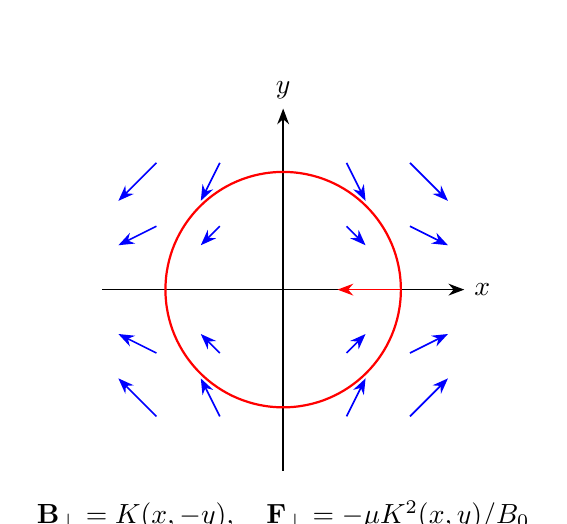
\begin{tikzpicture}[scale=1.15]
\draw[arr](-2,0)--(2,0)node[right]{$x$};\draw[arr](0,-2)--(0,2)node[above]{$y$};
\foreach \x in {-1.4,-.7,.7,1.4}{\foreach \y in {-1.4,-.7,.7,1.4}{\draw[arr,blue](\x,\y)--++({.3*\x},{-.3*\y});}}
\draw[red,thick](0,0)circle(1.3);\draw[arr,red](1.3,0)--(.6,0);
\node at(0,-2.5){$\mathbf B_\perp=K(x,-y),\quad \mathbf F_\perp=-\mu K^2(x,y)/B_0$};
\end{tikzpicture}
}
\ifdim\wd\diagrambox>.88\linewidth
\sbox{\diagrambox}{\resizebox{.88\linewidth}{!}{\usebox{\diagrambox}}}\fi
\ifdim\ht\diagrambox>.38\textheight
\resizebox{!}{.38\textheight}{\usebox{\diagrambox}}
\else\usebox{\diagrambox}\fi
\par\smallskip{\small 局部四极场及低场寻求原子的恢复力\par}\endgroup\end{minipage}\end{center}

外加 \(B_0\) 使原点总场不为零，势能的尖点变成平滑的二次极小值。题给
\(\mu>0\) 的原子倾向于低场区，故原点附近受到向中心的恢复力。

远处四根导线的电流代数和为零，导线场衰减，势能又趋向
\(\mu B_0\)。所以从原点向外，势能先升高、后降低，形成有限势垒，而不是永远增大。

\subsection{四、解题入口}\label{ux56dbux89e3ux9898ux5165ux53e3-3}

先把四根导线的坐标和电流符号列表，不要凭图形直接猜每个分量。线性项可用雅可比矩阵求，也可由场的有理表达式展开。

第三问先写 \(\sqrt{B_0^2+B_\perp^2}\)，再在 \(B_\perp/B_0\ll1\)
下展开。第四问求轴上极值只是第一步，还要说明任意逃逸路径不可能绕过更低的势垒。

下面用复数表达式把固定半径上场强的角度依赖写清楚，这给出最容易逃逸路径的证明，不只依靠``由对称性看起来应该沿轴''。

\subsection{五、解析}\label{ux4e94ux89e3ux6790-3}

\subsubsection{1.
精确空间分布}\label{ux7cbeux786eux7a7aux95f4ux5206ux5e03}

记

\[
C_I=\frac{\mu_0 I}{2\pi},\qquad
D_j=(x-x_j)^2+(y-y_j)^2,
\]

\[
(s_1,s_2,s_3,s_4)=(-1,+1,-1,+1).
\]

则导线总场为

\[
\boxed{\mathbf B_\perp=C_I\sum_{j=1}^4
s_j\frac{-(y-y_j)\mathbf i+(x-x_j)\mathbf j}{D_j}}.
\]

这就是导线外任意 \((x,y,z)\) 的精确空间分布，且
\(\partial\mathbf B_\perp/\partial z=0\)。若需要逐项分量，

\[
\frac{B_x}{C_I}
=\frac{y-a}{D_1}-\frac{y-a}{D_2}
+\frac{y+a}{D_3}-\frac{y+a}{D_4},
\]

\[
\frac{B_y}{C_I}
=-\frac{x+a}{D_1}+\frac{x-a}{D_2}
-\frac{x-a}{D_3}+\frac{x+a}{D_4}.
\]

导线位置处模型发散，公式只适用于导线外。外加场不属于导线电流产生的场，第一问不应把
\(B_0\) 混入 \(B_x,B_y\)。

\subsubsection{2.
紧凑的复数表达}\label{ux7d27ux51d1ux7684ux590dux6570ux8868ux8fbe}

令 \(z_c=x+iy\)，并定义

\[
\mathcal B=B_x-iB_y.
\]

单根导线场可写成 \(-iC_Is_j/(z_c-z_j)\)。对四根导线求和、通分后，

\[
\boxed{\mathcal B=
\frac{4\mu_0Ia^2}{\pi}
\frac{z_c}{z_c^4+4a^4}}.
\]

分母的四个零点正是四根导线所在的角点。近原点的分子正比于
\(z_c\)，远处则按 \(z_c^{-3}\) 衰减。

这一式不能与 \(B_x+iB_y\) 混用；虚部的负号是为了让直导线表达式成为
\(1/(z_c-z_j)\) 的形式。改变复数定义后，近场方向也会相应改变。

\subsubsection{3.
原点附近的线性场}\label{ux539fux70b9ux9644ux8fd1ux7684ux7ebfux6027ux573a}

当 \(|x|,|y|\ll a\)，

\[
\mathcal B\simeq\frac{\mu_0I}{\pi a^2}z_c.
\]

因此记

\[
K=\frac{\mu_0 I}{\pi a^2},
\]

便有

\[
\boxed{\mathbf B_\perp\simeq K(x\mathbf i-y\mathbf j)}.
\]

原点场为零，\(x,y\)
两方向梯度符号相反。四重对称性使接下来的非线性修正从五次项开始：

\[
\mathcal B=Kz_c\left(1-\frac{z_c^4}{4a^4}+\cdots\right).
\]

线性场满足 \(\nabla\cdot\mathbf B=K-K=0\)；在无电流的中心区域也满足
\(\nabla\times\mathbf B=0\)。两项检查能发现电流方向或符号误写。

\subsubsection{4.
势能展开与磁力}\label{ux52bfux80fdux5c55ux5f00ux4e0eux78c1ux529b}

总场的模为

\[
|\mathbf B_{\rm tot}|\simeq
\sqrt{B_0^2+K^2(x^2+y^2)}.
\]

令 \(\rho^2=x^2+y^2\)。在 \(K\rho\ll B_0\) 时，

\[
V\simeq\mu B_0+\frac{\mu K^2}{2B_0}\rho^2.
\]

所以

\[
\boxed{\mathbf F=-\nabla V
\simeq-\frac{\mu K^2}{B_0}(x\mathbf i+y\mathbf j)}.
\]

\(F_z=0\)，意味着这个无限长导线模型只在横向束缚，沿 \(z\)
没有势垒；题目第四问明确限定在 \(xy\) 平面内。

若只要求 \(\rho\ll a\) 而不要求 \(K\rho\ll B_0\)，还可保留

\[
\mathbf F\simeq-\mu
\frac{K^2(x\mathbf i+y\mathbf j)}
{\sqrt{B_0^2+K^2\rho^2}}.
\]

它是线性近场模型中的非谐力，不能再称为严格简谐恢复力。

\subsubsection{5.
两个近似条件的区别}\label{ux4e24ux4e2aux8fd1ux4f3cux6761ux4ef6ux7684ux533aux522b}

\(\rho\ll a\) 用于线性化导线场；\(K\rho\ll B_0\)
用于把场的模展开为二次势。外加场越弱，后一个条件可能比前一个更严格。

若原子质量为 \(m_a\)，二次势对应

\[
\omega_{\rm trap}
=\sqrt{\frac{\mu K^2}{m_aB_0}}.
\]

直接令 \(B_0\to0\)
会使这个频率形式上发散，但实际简谐近似的空间范围同时趋于零。零偏置时势能近中心为
\(\mu K\rho\)，存在尖点，并非无限刚度的简谐阱。

\subsubsection{6.
固定半径上的最小场强}\label{ux56faux5b9aux534aux5f84ux4e0aux7684ux6700ux5c0fux573aux5f3a}

在极坐标 \(z_c=\rho e^{i\varphi}\) 下，

\[
|\mathbf B_\perp|=
\frac{4\mu_0Ia^2\rho/\pi}
{\sqrt{\rho^8+8a^4\rho^4\cos4\varphi+16a^8}}.
\]

对固定 \(\rho\)，分子固定，分母在 \(\cos4\varphi=1\)
时最大。因此场强和势能在四条坐标半轴上最小：

\[
\varphi=0,\frac\pi2,\pi,\frac{3\pi}2.
\]

这些方向恰好位于相邻导线之间，而不是朝着导线角点。它们提供同样低的逃逸通道。

沿正 \(x\) 轴，

\[
B_x(x,0)=\frac{4\mu_0Ia^2x}{\pi(x^4+4a^4)},
\qquad B_y(x,0)=0.
\]

\subsubsection{7.
轴上势垒位置}\label{ux8f74ux4e0aux52bfux5792ux4f4dux7f6e}

对轴上场强求导，

\[
\frac{d}{dx}\frac{x}{x^4+4a^4}
=\frac{4a^4-3x^4}{(x^4+4a^4)^2}.
\]

正半轴的极大值位置为

\[
x_b=a\left(\frac43\right)^{1/4}.
\]

四个等价势垒位置为

\[
\boxed{(\pm x_b,0),\quad(0,\pm x_b)}.
\]

\begin{center}
\begin{minipage}{\linewidth}
\centering\begingroup\sbox{\diagrambox}{\small
\begin{tikzpicture}[xscale=1.1,yscale=2]
\draw[arr](0,0)--(6.6,0)node[right]{$\rho/a$};
\draw[arr](0,0)--(0,1.5)node[above]{$|\mathbf B_\perp|/(\mu_0I/\pi a)$};
\draw[blue,thick,domain=0:6,samples=120]plot(\x,{4*\x/(\x^4+4)});
\draw[dashed](1.07457,0)--(1.07457,.806);
\fill[red](1.07457,.806)circle(1.4pt)node[above right]{轴上鞍点};
\node at(3.8,1.15){固定半径时，轴向场最弱};
\end{tikzpicture}
}
\ifdim\wd\diagrambox>.88\linewidth
\sbox{\diagrambox}{\resizebox{.88\linewidth}{!}{\usebox{\diagrambox}}}\fi
\ifdim\ht\diagrambox>.38\textheight
\resizebox{!}{.38\textheight}{\usebox{\diagrambox}}
\else\usebox{\diagrambox}\fi
\par\smallskip{\small 轴上场强先增后减及鞍点位置\par}\endgroup\end{minipage}\end{center}

沿轴向经过这里，势能是最大值；在相同半径上偏离坐标轴，势能反而增大，所以它们是逃逸鞍点，而非整个平面的势能最大点。

在该处导线场强满足

\[
B_b^2=\frac{3\sqrt3}{8}
\left(\frac{\mu_0 I}{\pi a}\right)^2.
\]

\subsubsection{8.
为什么没有更低的绕行路径}\label{ux4e3aux4ec0ux4e48ux6ca1ux6709ux66f4ux4f4eux7684ux7ed5ux884cux8defux5f84}

任何从原点逃到无穷远的连续平面路径，都必须穿过半径为 \(x_b\)
的圆。在这个圆上，轴上点的势能最小，其值为

\[
V_b=\mu\sqrt{B_0^2+B_b^2}.
\]

因此任何逃逸路径的最大势能至少为
\(V_b\)。另一方面，沿任一坐标半轴向外，势能最大值恰好等于
\(V_b\)。这就同时给出了下界和实现下界的路径。

所以原点出发的最小逃逸动能为

\[
\boxed{K_{\min}=
\mu\left[
\sqrt{B_0^2+\frac{3\sqrt3}{8}
\left(\frac{\mu_0I}{\pi a}\right)^2}
-B_0\right]}.
\]

``刚能逃出''是能量阈值的极限说法：动能恰好等于阈值时，到达鞍点的速度趋于零，通常需要无限时间；实际穿越需略高于此阈值。

\subsubsection{9.
势垒的极限检查}\label{ux52bfux5792ux7684ux6781ux9650ux68c0ux67e5}

当 \(B_b\ll B_0\)，

\[
K_{\min}\simeq\frac{\mu B_b^2}{2B_0}.
\]

当 \(B_0\to0^+\)，

\[
K_{\min}\to\mu B_b.
\]

两式分别检验二次展开和无偏置极限。远处
\(V\to\mu B_0\)，等于原点势能，但逃出仍需要克服中间势垒；仅比较初末势能会错误地得到零逃逸能量。

\subsubsection{10.
鞍点附近的运动与阈值含义}\label{ux978dux70b9ux9644ux8fd1ux7684ux8fd0ux52a8ux4e0eux9608ux503cux542bux4e49}

沿正 \(x\) 轴，令 \(u=x/a\)，以及 \(S=\mu_0I/(\pi a)\)，则

\[
B_\perp=S\,b(u),\qquad b(u)=\frac{4u}{u^4+4}.
\]

在 \(u_b=(4/3)^{1/4}\) 有 \(b'(u_b)=0\)，并可计算

\[
b(u_b)b''(u_b)=-\frac{27}{16}.
\]

因此势能在逃逸鞍点的轴向二阶导数为

\[
V''(x_b)=-\frac{27\mu S^2}
{16a^2\sqrt{B_0^2+B_b^2}}<0.
\]

若原子质量为 \(m_a\)，在 \(\xi=x-x_b\) 很小时，

\[
\ddot\xi\simeq\Lambda^2\xi,\qquad
\Lambda^2=-\frac{V''(x_b)}{m_a}>0.
\]

这与原点附近的简谐方程符号相反：原点扰动被拉回，鞍点轴向扰动被推开。

当总能量恰为 \(V_b\)，从内侧接近鞍点时 \(\dot\xi\simeq-\Lambda\xi\)，故
\(\xi\) 指数趋向零、到达时间无穷。若能量为 \(V_b+\delta E\)，则

\[
\dot\xi^2\simeq
\frac{2\delta E}{m_a}+\Lambda^2\xi^2.
\]

正的 \(\delta E\)
允许有限时间穿越。它说明第四问的``最小动能''是穿越能量的下确界；实际逃逸需稍高于阈值，但这不改变所求势垒公式。

\clearpage

\section{第 5 题
旋转参考系与经典塞曼分裂（40分）}\label{ux7b2c-5-ux9898-ux65cbux8f6cux53c2ux8003ux7cfbux4e0eux7ecfux5178ux585eux66fcux5206ux88c240ux5206}

假定原子中的价电子质量为 \(m\)，电荷为
\(-e\)（\(e>0\)），受到指向原子中心的各向同性线性回复力
\(-m\omega_0^2\mathbf r\)，无磁场时作固有圆频率为 \(\omega_0\)
的简谐振动，并发出圆频率为 \(\omega_0\) 的光。

现在原子置于沿 \(+z\) 方向的均匀磁场中，磁感应强度大小为
\(B\)。为方便，把磁场参数化为

\[
B=\frac{2m}{e}\omega_L.
\]

（1）选择绕磁场方向匀角速转动的参考系，使电子在该参考系中做简谐振动，写出直角坐标中的动力学分量方程并求解。

（2）把第一问的解变换到实验室参考系的直角坐标。

（3）证明原来的谱线在磁场中分成三条；在弱磁场 \(\omega_L\ll\omega_0\)
时求三条谱线的频率间隔。

已知：转动角速度为 \(\boldsymbol\Omega\)
的参考系中，电子除受惯性离心力外，还受科里奥利力；若相对速度为
\(\mathbf v'\)，科里奥利力为 \(-2m\boldsymbol\Omega\times\mathbf v'\)。

\subsection{一、题型定位}\label{ux4e00ux9898ux578bux5b9aux4f4d-4}

选取旋转参考系消除速度耦合，再把旋转系中的振动变换成实验室中的两个横向圆偏振模。沿磁场的纵向振动保持原频率，横向两个模的频率分开。

``电子在旋转系中做简谐振动''是指各直角坐标满足简谐方程；一般轨迹可以是椭圆，不一定是一条径向直线。求通解时必须保留足够的初始条件常数。

\subsection{二、知识点}\label{ux4e8cux77e5ux8bc6ux70b9-4}

在实验室中，电子满足

\[
m\ddot{\mathbf r}=-m\omega_0^2\mathbf r
-e\dot{\mathbf r}\times B\mathbf k.
\]

电子电荷的负号决定耦合项方向。由叉积得

\[
\ddot x=-\omega_0^2x-2\omega_L\dot y,
\]

\[
\ddot y=-\omega_0^2y+2\omega_L\dot x,\qquad
\ddot z=-\omega_0^2z.
\]

磁力垂直速度，不做功，故实验室中的机械能

\[
\mathcal E=\frac m2
\left(\dot x^2+\dot y^2+\dot z^2
+\omega_0^2(x^2+y^2+z^2)\right)
\]

恒定。磁场改变运动模的频率，并不要求给电子输入持续能量。

\subsection{三、物理图像}\label{ux4e09ux7269ux7406ux56feux50cf-4}

\begin{center}
\begin{minipage}{\linewidth}
\centering\begingroup\sbox{\diagrambox}{\small
\begin{tikzpicture}[scale=.95]
\draw[arr](0,0)--(3.5,0)node[right]{$x$};\draw[arr](0,0)--(0,3.5)node[above]{$y$};
\draw[arr,blue](0,0)--(2.9,1.68)node[right]{$x'$};
\draw[arr,blue](0,0)--(-1.68,2.9)node[above]{$y'$};
\draw[arr](1,0)arc(0:30:1)node[midway,right]{$\omega_Lt$};
\node at(4,2.5){$\boldsymbol\Omega=\omega_L\mathbf k$};
\node at(3,-1){$\mathbf v=\mathbf v'+\boldsymbol\Omega\times\mathbf r$};
\end{tikzpicture}
}
\ifdim\wd\diagrambox>.88\linewidth
\sbox{\diagrambox}{\resizebox{.88\linewidth}{!}{\usebox{\diagrambox}}}\fi
\ifdim\ht\diagrambox>.38\textheight
\resizebox{!}{.38\textheight}{\usebox{\diagrambox}}
\else\usebox{\diagrambox}\fi
\par\smallskip{\small 实验室坐标与沿正磁场方向转动的坐标\par}\endgroup\end{minipage}\end{center}

选择旋转系以 \(\omega_L\) 沿 \(+z\)
转动。它的科里奥利力恰好抵消相对运动产生的磁力；但还有由参考系整体旋转产生的磁力和离心力，二者相加后改变横向回复力。

因此旋转系的横向频率不是严格的 \(\omega_0\)，而是
\(\sqrt{\omega_0^2+\omega_L^2}\)。弱磁场时这个改变属于二阶小量，但前两问并未允许把它提前删掉。

\begin{center}
\begin{minipage}{\linewidth}
\centering\begingroup\sbox{\diagrambox}{\small
\begin{tikzpicture}[scale=.95]
\foreach \xx/\lab/\ang in {0/{\Omega_\perp+\omega_L}/55,4/{\Omega_\perp-\omega_L}/-55}
{\begin{scope}[shift={(\xx,0)}]
\draw[blue,thick](0,0)circle(1.3);\draw[arr](1.3,0)arc(0:\ang:1.3);
\draw[arr,gray](-1.7,0)--(1.7,0);\draw[arr,gray](0,-1.7)--(0,1.7);
\node at(0,-2.1){$\lab$};\end{scope}}
\node at(2,2.2){两个相反旋向的横向圆运动};
\end{tikzpicture}
}
\ifdim\wd\diagrambox>.88\linewidth
\sbox{\diagrambox}{\resizebox{.88\linewidth}{!}{\usebox{\diagrambox}}}\fi
\ifdim\ht\diagrambox>.38\textheight
\resizebox{!}{.38\textheight}{\usebox{\diagrambox}}
\else\usebox{\diagrambox}\fi
\par\smallskip{\small 两个横向本征模有相反旋向\par}\endgroup\end{minipage}\end{center}

实验室中可把一般横向运动分解为两个相反旋向的圆运动。每个圆运动在 \(x,y\)
上有同一频率、相差四分之一周期；两模频率不同，叠加后形成一般轨迹。

\subsection{四、解题入口}\label{ux56dbux89e3ux9898ux5165ux53e3-4}

先把旋转系中的速度关系写全：

\[
\mathbf v=\mathbf v'+\boldsymbol\Omega\times\mathbf r.
\]

再把实验室磁力换成相对速度项和位置项，最后加科里奥利力与离心力。若只把磁力中的
\(\mathbf v\) 换成 \(\mathbf v'\)，会漏掉横向频率的二阶修正。

求解采用直角坐标通解最稳妥；变换到实验室后，可用积化和差或复数
\(u=x+iy\) 识别两个频率。复数法还提供一条独立的本征频率验证。

\subsection{五、解析}\label{ux4e94ux89e3ux6790-4}

\subsubsection{1.
旋转系中的完整动力学方程}\label{ux65cbux8f6cux7cfbux4e2dux7684ux5b8cux6574ux52a8ux529bux5b66ux65b9ux7a0b}

设 \(\boldsymbol\Omega=\Omega\mathbf k\)。在旋转系中，

\[
m\ddot{\mathbf r}'=-m\omega_0^2\mathbf r
-e(\mathbf v'+\boldsymbol\Omega\times\mathbf r)\times B\mathbf k
-2m\boldsymbol\Omega\times\mathbf v'
-m\boldsymbol\Omega\times(\boldsymbol\Omega\times\mathbf r).
\]

其中坐标矢量 \(\mathbf r\)
在两系表示不同，但几何矢量相同。磁力的速度部分为

\[
-e\mathbf v'\times B\mathbf k
=2m\omega_L\mathbf k\times\mathbf v'.
\]

它与科里奥利力合并后是

\[
2m(\omega_L-\Omega)\mathbf k\times\mathbf v'.
\]

因此取

\[
\boxed{\boldsymbol\Omega=\omega_L\mathbf k}
\]

消去速度耦合。旋转方向沿 \(+z\)，与电子的负电荷及给定磁场方向相适应。

\subsubsection{2.
位置项与旋转系通解}\label{ux4f4dux7f6eux9879ux4e0eux65cbux8f6cux7cfbux901aux89e3}

设
\(\mathbf r_\perp=x'\mathbf i'+y'\mathbf j'\)。参考系旋转所带来的磁力为
\(-2m\omega_L^2\mathbf r_\perp\)，离心力为
\(+m\omega_L^2\mathbf r_\perp\)，合计为
\(-m\omega_L^2\mathbf r_\perp\)。

于是令

\[
\Omega_\perp=\sqrt{\omega_0^2+\omega_L^2},
\]

旋转系分量方程为

\[
\boxed{\ddot x'+\Omega_\perp^2x'=0,\quad
\ddot y'+\Omega_\perp^2y'=0,\quad
\ddot z'+\omega_0^2z'=0}.
\]

完整通解为

\[
x'=a_x\cos\Omega_\perp t+b_x\sin\Omega_\perp t,
\]

\[
y'=a_y\cos\Omega_\perp t+b_y\sin\Omega_\perp t,
\]

\[
z'=a_z\cos\omega_0t+b_z\sin\omega_0t.
\]

六个实常数由三维初始位置和速度决定。\(x',y'\)
的振幅和相位一般不同，所以横向轨迹通常为椭圆。

\subsubsection{3.
初始条件的变换}\label{ux521dux59cbux6761ux4ef6ux7684ux53d8ux6362}

令 \(t=0\) 时两组坐标轴重合。若实验室初始坐标是
\((x_0,y_0,z_0)\)，初始速度是 \((v_{x0},v_{y0},v_{z0})\)，则

\[
(a_x,a_y,a_z)=(x_0,y_0,z_0),
\]

\[
b_x=\frac{v_{x0}+\omega_Ly_0}{\Omega_\perp},
\qquad b_y=\frac{v_{y0}-\omega_Lx_0}{\Omega_\perp},
\qquad b_z=\frac{v_{z0}}{\omega_0}.
\]

即使实验室初速度为零，旋转系初速度也未必为零。一个离轴静止电子，在旋转坐标中本来就具有相反方向的表观速度。

\subsubsection{4.
变回实验室坐标}\label{ux53d8ux56deux5b9eux9a8cux5ba4ux5750ux6807}

坐标变换为

\[
\boxed{x=x'\cos\omega_Lt-y'\sin\omega_Lt},
\]

\[
\boxed{y=x'\sin\omega_Lt+y'\cos\omega_Lt,\quad z=z'}.
\]

代入上一节通解，即得到第二问的完整解。例如

\[
\begin{aligned}
x={}&(a_x\cos\Omega_\perp t+b_x\sin\Omega_\perp t)\cos\omega_Lt\\
&-(a_y\cos\Omega_\perp t+b_y\sin\Omega_\perp t)\sin\omega_Lt,
\end{aligned}
\]

\[
\begin{aligned}
y={}&(a_x\cos\Omega_\perp t+b_x\sin\Omega_\perp t)\sin\omega_Lt\\
&+(a_y\cos\Omega_\perp t+b_y\sin\Omega_\perp t)\cos\omega_Lt.
\end{aligned}
\]

这两个式子适用于任意初始条件，不需要假定两方向相位相同，也不需要假定电子在旋转系里径向振动。

\subsubsection{5.
用复数识别本征频率}\label{ux7528ux590dux6570ux8bc6ux522bux672cux5f81ux9891ux7387}

令 \(u=x+iy\)。实验室耦合方程化为

\[
\ddot u-2i\omega_L\dot u+\omega_0^2u=0.
\]

设 \(u=e^{i\omega_Lt}w\)，代入后得到

\[
\ddot w+\Omega_\perp^2w=0.
\]

因此

\[
\boxed{u=c_+e^{i(\Omega_\perp+\omega_L)t}
+c_-e^{-i(\Omega_\perp-\omega_L)t}}.
\]

\(c_+,c_-\)
为两个任意复常数，共四个实自由度，正好对应横向初始条件。两个指数的符号相反，说明两个圆运动的旋向相反。

定义

\[
\omega_+=\Omega_\perp+\omega_L,\qquad
\omega_-=\Omega_\perp-\omega_L.
\]

二者都为正，且

\[
\omega_+\omega_-=\omega_0^2,\qquad
\omega_+-\omega_-=2\omega_L.
\]

这两个恒等式是本征频率的直接检查。

\subsubsection{6.
三条可能的谱线}\label{ux4e09ux6761ux53efux80fdux7684ux8c31ux7ebf}

沿磁场的振动频率保持 \(\omega_0\)；横向运动包含 \(\omega_-,\omega_+\)
两个频率。因此在一般初始条件下，辐射包含

\[
\boxed{\omega_-,\quad\omega_0,\quad\omega_+}.
\]

\begin{center}
\begin{minipage}{\linewidth}
\centering\begingroup\sbox{\diagrambox}{\small
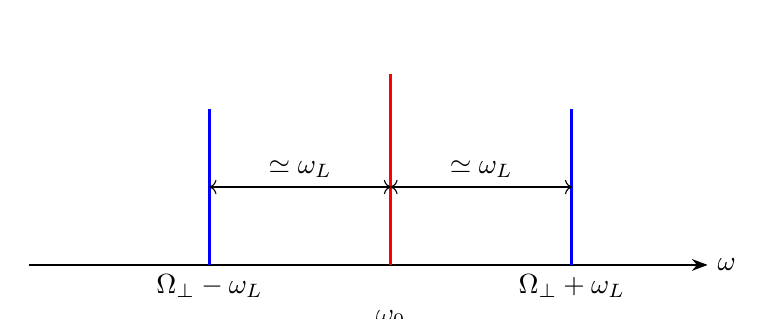
\begin{tikzpicture}[xscale=1.15,yscale=.9]
\draw[arr](0,0)--(7.5,0)node[right]{$\omega$};
\draw[very thick,blue](2,0)--(2,2.2);\draw[very thick,red](4,0)--(4,2.7);
\draw[very thick,blue](6,0)--(6,2.2);
\node[below]at(2,0){$\Omega_\perp-\omega_L$};\node[below]at(4,-.5){$\omega_0$};\node[below]at(6,0){$\Omega_\perp+\omega_L$};
\draw[<->](2,1.1)--(4,1.1)node[midway,above]{$\simeq\omega_L$};
\draw[<->](4,1.1)--(6,1.1)node[midway,above]{$\simeq\omega_L$};
\end{tikzpicture}
}
\ifdim\wd\diagrambox>.88\linewidth
\sbox{\diagrambox}{\resizebox{.88\linewidth}{!}{\usebox{\diagrambox}}}\fi
\ifdim\ht\diagrambox>.38\textheight
\resizebox{!}{.38\textheight}{\usebox{\diagrambox}}
\else\usebox{\diagrambox}\fi
\par\smallskip{\small 三条谱线及弱场间隔\par}\endgroup\end{minipage}\end{center}

严格地说，三条是该经典模型允许的三个频率。某一特殊初始条件可能使一个模的振幅为零；某一观察方向也可能看不到某个偏振分量。频率结构不等于任意一次单电子运动都必然同时显示三条等强谱线。

若观察方向沿
\(z\)，纵向偶极振动不向自身轴向辐射，因此只见两个横向圆偏振频率；若从侧面观察，纵向中央线和横向边线均可出现。该补充有助于区分动力学频率与观测强度。

\subsubsection{7.
弱磁场的频率间隔}\label{ux5f31ux78c1ux573aux7684ux9891ux7387ux95f4ux9694}

当 \(\omega_L\ll\omega_0\)，

\[
\Omega_\perp
=\omega_0+\frac{\omega_L^2}{2\omega_0}
+O\!\left(\frac{\omega_L^4}{\omega_0^3}\right).
\]

保留一阶项，

\[
\omega_\pm\simeq\omega_0\pm\omega_L.
\]

故相邻谱线的圆频率间隔约为

\[
\boxed{\Delta\omega\simeq\omega_L=\frac{eB}{2m}}.
\]

若``频率''采用每秒周期数 \(\nu=\omega/(2\pi)\)，则

\[
\boxed{\Delta\nu\simeq\frac{\omega_L}{2\pi}
=\frac{eB}{4\pi m}}.
\]

两侧线的精确圆频率差恒为
\(2\omega_L\)；但中央线并非两边线精确中点。严格的两相邻间隔分别为

\[
\omega_+-\omega_0=\omega_L+\Omega_\perp-\omega_0,
\]

\[
\omega_0-\omega_-=\omega_L-(\Omega_\perp-\omega_0).
\]

\subsubsection{8.
一般角动量常数不能设为零}\label{ux4e00ux822cux89d2ux52a8ux91cfux5e38ux6570ux4e0dux80fdux8bbeux4e3aux96f6}

参考解答的部分极坐标路线把一个积分常数以``任意半径都成立''为由设为零。这个推论对一般初始条件不成立。

由实验室极坐标的角向方程可得

\[
\rho^2(\dot\varphi-\omega_L)=C.
\]

在旋转系中，\(\varphi'=\varphi-\omega_Lt\)，所以

\[
\rho^2\dot\varphi'=C.
\]

\(C\)
是旋转系横向运动的比角动量，由初始条件决定；没有理由对所有初始条件都等于零。只有特殊的直线振动才有
\(C=0\)。

一般情况下径向方程是

\[
\ddot\rho-\frac{C^2}{\rho^3}
=-\Omega_\perp^2\rho.
\]

它包含离心项，而 \(x',y'\)
仍分别是简谐振动。使用直角坐标通解即可完整解决原题，避免把特殊径向运动误写为所有运动。

\subsubsection{9.
零场与强场检查}\label{ux96f6ux573aux4e0eux5f3aux573aux68c0ux67e5}

令 \(B\to0\)，有 \(\omega_L\to0\)，三个频率都回到
\(\omega_0\)，恢复原来的简并振动。

在 \(\omega_L\gg\omega_0\) 的形式极限中，

\[
\omega_+\simeq2\omega_L,\qquad
\omega_-\simeq\frac{\omega_0^2}{2\omega_L}.
\]

低频始终为正，因为 \(\Omega_\perp>\omega_L\)。如果提前用
\(\omega_0-\omega_L\)
代替精确低频，强场下会得到负值，说明弱场近似已经越界。

\clearpage

\section{第 6 题
同心球系统的导热与灰体辐射交换（40分）}\label{ux7b2c-6-ux9898-ux540cux5fc3ux7403ux7cfbux7edfux7684ux5bfcux70edux4e0eux7070ux4f53ux8f90ux5c04ux4ea4ux636240ux5206}

太空中的装置由同心内球和球壳构成，内球到球壳内表面之间为真空。内球半径
\(r=0.200\,\mathrm m\)，温度恒定，比辐射率 \(e=0.800\)。球壳导热系数

\[
\kappa=1.00\times10^{-2}\,
\mathrm{J\,m^{-1}s^{-1}K^{-1}},
\]

内、外半径分别为
\(R_1=0.900\,\mathrm m\)、\(R_2=1.00\,\mathrm m\)。各表面的热辐射各向同性，球壳外表面可看作黑体。装置处于热稳定状态，球壳内表面比辐射率
\(E=0.800\)。

斯特藩常量为
\(\sigma=5.67\times10^{-8}\,\mathrm{W\,m^{-2}K^{-4}}\)，宇宙微波背景辐射温度为
\(T_b=2.73\,\mathrm K\)。若单位时间内由内球传到球壳外表面的净热量为
\(Q=44.0\,\mathrm W\)，求：

（1）球壳外表面温度 \(T_2\)；（2）球壳内表面温度 \(T_1\)；（3）内球温度
\(T_0\)。

已知：比辐射率是表面发射功率与同温黑体发射功率之比；吸收比是吸收功率与入射功率之比。物体同温下的吸收比等于比辐射率。沿热流方向每单位长度温度梯度为
\(dT/dz\) 时，单位面积热流为 \(-\kappa\,dT/dz\)。

\begin{center}
\begin{minipage}{\linewidth}
\centering\begingroup\sbox{\diagrambox}{\small
\begin{tikzpicture}[scale=.9]
\fill[gray!15](0,0)circle(2.5);\fill[white](0,0)circle(2.1);\fill[blue!15](0,0)circle(.55);
\draw[thick](0,0)circle(2.5);\draw[thick](0,0)circle(2.1);\draw[thick](0,0)circle(.55);
\draw[arr](0,0)--(.39,.39)node[above]{$r$};
\draw[arr](0,0)--(-1.82,1.05)node[midway,above]{$R_1$};
\draw[arr](0,0)--(2.16,-1.25)node[midway,below]{$R_2$};
\node at(0,-.25){$T_0$};\node at(-2.9,0){$T_1$};\node at(2.9,0){$T_2$};
\node at(0,3.2){真空层：辐射；球壳：导热；外界$T_b$};
\end{tikzpicture}
}
\ifdim\wd\diagrambox>.88\linewidth
\sbox{\diagrambox}{\resizebox{.88\linewidth}{!}{\usebox{\diagrambox}}}\fi
\ifdim\ht\diagrambox>.38\textheight
\resizebox{!}{.38\textheight}{\usebox{\diagrambox}}
\else\usebox{\diagrambox}\fi
\par\smallskip{\small 同心球、真空层和导热球壳\par}\endgroup\end{minipage}\end{center}

\subsection{一、题型定位}\label{ux4e00ux9898ux578bux5b9aux4f4d-5}

装置处于稳态：内球与球壳内表面通过辐射交换，球壳内外表面通过导热传热，外表面向宇宙背景净辐射。三个环节的净功率都是
\(Q\)，但温度关系各不相同。

第三问不能只计算内球首次发射后被球壳吸收的比例。球壳内表面是凹面，反射或发射的一部分辐射会再次照到球壳自身；这部分会继续反射或被吸收，必须计入。

\subsection{二、知识点}\label{ux4e8cux77e5ux8bc6ux70b9-5}

外表面是黑体，净辐射功率为发射减吸收：

\[
Q_{\rm out}=4\pi R_2^2\sigma(T_2^4-T_b^4).
\]

球壳稳态径向导热的净功率为

\[
Q=-4\pi R^2\kappa\frac{dT}{dR}.
\]

灰体辐射交换需要区分三个量：表面自身发射功率密度
\(\epsilon\sigma T^4\)，入射辐照度
\(G\)，以及包括发射和反射在内的出射辐射度 \(J\)：

\[
J=\epsilon\sigma T^4+(1-\epsilon)G.
\]

这三个量单位均为 \(\mathrm{W/m^2}\)。净向外功率密度是 \(J-G\)，不能把
\(J\) 本身当成净流。

\subsection{三、物理图像}\label{ux4e09ux7269ux7406ux56feux50cf-5}

由稳态条件，沿传热方向必有
\(T_0>T_1>T_2>T_b\)。球壳内外表面温差由导热热阻决定；真空层没有导热温度梯度，它是两个表面的辐射耦合。

\begin{center}
\begin{minipage}{\linewidth}
\centering\begingroup\sbox{\diagrambox}{\small
\begin{tikzpicture}[xscale=2.8,yscale=.021]
\draw[arr](.15,70)--(1.15,70)node[right]{$R$};
\draw[arr](.15,70)--(.15,260)node[above]{$T/{\rm K}$};
\fill(.2,216.906)circle(.9pt)node[right]{$T_0$};
\draw[thick,blue,domain=.9:1,samples=30]plot(\x,{88.64+350.14*(1/\x-1)});
\fill(.9,127.55)circle(.9pt)node[above left]{$T_1$};\fill(1,88.64)circle(.9pt)node[above right]{$T_2$};
\node at(.55,175){真空中没有物质温度曲线};
\end{tikzpicture}
}
\ifdim\wd\diagrambox>.88\linewidth
\sbox{\diagrambox}{\resizebox{.88\linewidth}{!}{\usebox{\diagrambox}}}\fi
\ifdim\ht\diagrambox>.38\textheight
\resizebox{!}{.38\textheight}{\usebox{\diagrambox}}
\else\usebox{\diagrambox}\fi
\par\smallskip{\small 球壳温度曲线和真空层的区别\par}\endgroup\end{minipage}\end{center}

内球为凸面，所有向外发射最终都碰到球壳内表面。球壳内表面向内发射则有两种目的地：内球和球壳自身其他位置。后者正是凹面自照项。

\begin{center}
\begin{minipage}{\linewidth}
\centering\begingroup\sbox{\diagrambox}{\small
\begin{tikzpicture}[scale=.85]
\draw[arr](0,0)--(10,0)node[right]{$Q/\sigma$};
\foreach \x/\lab in {0/T_0^4,3/{J_0/\sigma},6/{J_1/\sigma},9/T_1^4}{\fill(\x,0)circle(2pt);\node[above]at(\x,0){$\lab$};}
\foreach \x/\lab in {1.5/{(1-e)/(eA_0)},4.5/{1/A_0},7.5/{(1-E)/(EA_1)}}
{\draw[thick,fill=white](\x-.55,-.2)rectangle(\x+.55,.2);\node[below]at(\x,-.5){$\lab$};}
\node at(4.5,1.4){辐射电阻串联；流量为$Q/\sigma$};
\end{tikzpicture}
}
\ifdim\wd\diagrambox>.88\linewidth
\sbox{\diagrambox}{\resizebox{.88\linewidth}{!}{\usebox{\diagrambox}}}\fi
\ifdim\ht\diagrambox>.38\textheight
\resizebox{!}{.38\textheight}{\usebox{\diagrambox}}
\else\usebox{\diagrambox}\fi
\par\smallskip{\small 两灰体表面与空间的辐射电阻\par}\endgroup\end{minipage}\end{center}

图中各电阻表示辐射度关系的代数结构，不是物体的电学电阻。流量对应
\(Q/\sigma\)，势差对应温度四次方。表面电阻与面积有关，不能把两个比辐射率简单相乘。

\subsection{四、解题入口}\label{ux56dbux89e3ux9898ux5165ux53e3-5}

按热流从外向内求解：先由外部净辐射求 \(T_2\)；再由球壳导热求
\(T_1\)；最后由同心灰体的完整辐射交换求 \(T_0\)。

第三步先写视角因子。记内球表面积 \(A_0=4\pi r^2\)，球壳内表面积
\(A_1=4\pi R_1^2\)，以及

\[
f=\frac{A_0}{A_1}=\frac{r^2}{R_1^2}.
\]

内球到球壳的视角因子为1；由互易关系，球壳到内球的视角因子为
\(f\)；球壳到自身的视角因子为
\(1-f\)。以下默认题给各向同性辐射对应漫辐射、漫反射的灰体模型。

\subsection{五、解析}\label{ux4e94ux89e3ux6790-5}

\subsubsection{1.
外表面净辐射}\label{ux5916ux8868ux9762ux51c0ux8f90ux5c04}

热稳定要求外表面净散热等于 \(Q\)，所以

\[
Q=4\pi R_2^2\sigma(T_2^4-T_b^4).
\]

解得

\[
\boxed{T_2=\left(T_b^4+
\frac{Q}{4\pi R_2^2\sigma}\right)^{1/4}}.
\]

代入数值，

\[
\boxed{T_2=88.6472\,\mathrm K\simeq88.6\,\mathrm K}.
\]

背景项在这里很小，但写出它才能保证 \(Q=0\) 时装置趋于
\(T_b\)，而不是不合理地趋于绝对零度。因为题给的是净功率，不能仅用
\(Q=4\pi R_2^2\sigma T_2^4\) 当作精确关系。

\subsubsection{2.
球壳径向导热}\label{ux7403ux58f3ux5f84ux5411ux5bfcux70ed}

任何半径 \(R\) 上穿过球面的净功率均为 \(Q\)：

\[
\frac{dT}{dR}=-\frac{Q}{4\pi\kappa R^2}.
\]

从 \(R_1\) 积分到 \(R_2\)，

\[
T_2-T_1=-\frac{Q}{4\pi\kappa}
\int_{R_1}^{R_2}\frac{dR}{R^2}.
\]

因此

\[
\boxed{T_1=T_2+
\frac{Q}{4\pi\kappa}
\left(\frac1{R_1}-\frac1{R_2}\right)}.
\]

球壳导热热阻为

\[
\mathcal R_{\rm cond}=
\frac1{4\pi\kappa}\left(\frac1{R_1}-\frac1{R_2}\right).
\]

代入数值得

\[
T_1-T_2=38.9045\,\mathrm K,\qquad
\boxed{T_1=127.5517\,\mathrm K\simeq128\,\mathrm K}.
\]

若直接采用平板公式，必须选合适的等效面积；使用内表面积或外表面积中的任意一个，都会留下系统误差。

\subsubsection{3.
球壳内表面的自照}\label{ux7403ux58f3ux5185ux8868ux9762ux7684ux81eaux7167}

由几何互易关系，

\[
F_{0\to1}=1,\quad F_{0\to0}=0,
\]

\[
F_{1\to0}=f,\qquad F_{1\to1}=1-f.
\]

本题
\(f=(.2/.9)^2=0.0493827\)，因此球壳向内发射的绝大部分辐射并不直接打到内球，而是先打到球壳内表面其他位置。

这不会改变各表面温度均匀的假设，却会改变反射后的入射辐照度。只写
\(G_1=fJ_0\) 而省略 \((1-f)J_1\)，就漏掉自照。

完整入射关系为

\[
G_0=J_1,\qquad
G_1=fJ_0+(1-f)J_1.
\]

\subsubsection{4. 辐射度方程}\label{ux8f90ux5c04ux5ea6ux65b9ux7a0b}

两个灰体表面的出射辐射度分别满足

\[
J_0=e\sigma T_0^4+(1-e)J_1,
\]

\[
J_1=E\sigma T_1^4+(1-E)
\left[fJ_0+(1-f)J_1\right].
\]

净热流由内球流出，

\[
Q=A_0(J_0-J_1).
\]

从第一式可整理出

\[
\sigma T_0^4
=J_0+\frac{1-e}{e}\frac Q{A_0}.
\]

从第二式可整理出

\[
J_1=\sigma T_1^4+\frac{1-E}{E}\frac Q{A_1}.
\]

这一步利用 \(f(J_0-J_1)=Q/A_1\)，正是面积互易关系使净功率一致。

两式相减，得到

\[
\sigma(T_0^4-T_1^4)=
Q\left[\frac{1-e}{eA_0}
+\frac1{A_0}+\frac{1-E}{EA_1}\right].
\]

\subsubsection{5.
完整的灰体交换公式}\label{ux5b8cux6574ux7684ux7070ux4f53ux4ea4ux6362ux516cux5f0f}

将上一式整理，

\[
\boxed{
Q=\frac{A_0\sigma(T_0^4-T_1^4)}
{\displaystyle \frac1e+f\left(\frac1E-1\right)}}.
\]

定义无量纲辐射阻因子

\[
D=\frac1e+f\left(\frac1E-1\right).
\]

则

\[
\boxed{T_0=
\left[T_1^4+\frac{QD}{4\pi r^2\sigma}\right]^{1/4}}.
\]

本题

\[
D=1.25+0.0493827\times0.25=1.26234568.
\]

用未提前舍入的 \(T_1\) 计算，

\[
\boxed{T_0=216.9062\,\mathrm K\simeq217\,\mathrm K}.
\]

内球温度高于球壳内表面，净流方向与题意一致。

\subsubsection{6.
与参考答案的实质差异}\label{ux4e0eux53c2ux8003ux7b54ux6848ux7684ux5b9eux8d28ux5deeux5f02}

参考答案采用的反射级数没有计入球壳内表面到自身的反射链，得到的阻因子为

\[
D_{\rm ref}=
\frac{1-(1-e)(1-E)f}{eE}=1.55941358,
\]

从而算得约
\(227\,\mathrm K\)。在完整的漫辐射灰体模型下，该结果应修正为约
\(217\,\mathrm K\)。

这不是舍入差异。两者对 \(E\to0\)
的极限行为不同：完整模型在球壳内表面吸收比趋于零时交换热阻趋于无穷；漏项公式却可留下不合理的有限交换能力。

整理版保留原题数据，同时明确写出修正推导；参考解答中的 \(T_2,T_1\)
与完整模型相符，只有第三问需要修正。

\subsubsection{7.
用多次反射验证}\label{ux7528ux591aux6b21ux53cdux5c04ux9a8cux8bc1}

设一份辐射能量已碰到球壳内表面。球壳吸收比例为 \(E\)，反射比例为
\(1-E\)。反射后，比例 \(f\) 碰到内球，比例 \(1-f\) 再碰到球壳。

考虑所有可能的球壳自反射次数，最终返回内球的概率为

\[
P_{\rm return}
=(1-E)f\sum_{j=0}^{\infty}
\left[(1-E)(1-f)\right]^j
=\frac{(1-E)f}{E+(1-E)f}.
\]

内球吸收或反射后还会继续产生交换。内球自身发射的能量最终在球壳吸收的比例为

\[
\eta_{0\to1}
=\frac{1-P_{\rm return}}
{1-(1-e)P_{\rm return}}
=\frac{E}{E+e(1-E)f}.
\]

所以来自内球自身发射、最终被球壳吸收的功率为

\[
eA_0\sigma T_0^4\,\eta_{0\to1}.
\]

反方向按面积互易得到同一交换系数乘 \(T_1^4\)。两者作差，恰好恢复
\(Q=A_0\sigma(T_0^4-T_1^4)/D\)，与辐射度方程独立一致。

\subsubsection{8.
有用的极限检查}\label{ux6709ux7528ux7684ux6781ux9650ux68c0ux67e5}

若 \(E=1\)，球壳不反射，

\[
Q=eA_0\sigma(T_0^4-T_1^4).
\]

若 \(e=E=1\)，恢复两个黑体表面的交换。若 \(f\to0\) 且 \(E\)
为固定非零值，小内球面对大空腔，

\[
Q\to eA_0\sigma(T_0^4-T_1^4),
\]

因为空腔内表面的多次自反射使它的有效辐射环境趋近黑体。

若 \(f\to1\)，得到两个面积近乎相等灰体的熟悉因子

\[
D\to\frac1e+\frac1E-1.
\]

以上极限既检验面积因子，也检验是否保留凹面自照。

\subsubsection{9. 精度与单位}\label{ux7cbeux5ea6ux4e0eux5355ux4f4d}

本题用 SI 单位统一计算，温度四次方必须使用开尔文。\(\kappa\)
的题给单位等价于 \(\mathrm{W\,m^{-1}K^{-1}}\)，不是热容单位。

数值计算宜把 \(T_2,T_1\) 的内部精度保留到最后；若先把 \(T_1\) 舍入成128
K再求四次方，会产生可避免的误差。正式答案按题给三位有效数字给出
\(88.6\,\mathrm K,128\,\mathrm K,217\,\mathrm K\)。

\subsubsection{10.
辐射度数值与两侧净流检查}\label{ux8f90ux5c04ux5ea6ux6570ux503cux4e0eux4e24ux4fa7ux51c0ux6d41ux68c0ux67e5}

以未舍入温度计算，两个出射辐射度和入射辐照度为

\[
J_0=103.6241\,\mathrm{W/m^2},\quad
J_1=16.0889\,\mathrm{W/m^2},
\]

\[
G_0=16.0889\,\mathrm{W/m^2},\quad
G_1=20.4116\,\mathrm{W/m^2}.
\]

内球净向外功率为

\[
A_0(J_0-G_0)=44.0\,\mathrm W.
\]

球壳内表面净吸收功率为

\[
A_1(G_1-J_1)=44.0\,\mathrm W.
\]

两侧净功率完全相同，说明视角因子、表面积和反射项保持整体能量守恒。球壳入射辐照度高于自身出射辐射度，因此净吸收；它并不要求球壳自身完全不发射。

另外，灰体内球自身发射功率是 \(eA_0\sigma T_0^4\)，一般大于44
W，因为内球同时吸收空腔辐射。只有发射减去吸收才是外加热源需要持续补充的净功率。

采用参考答案的227 K代入完整方程，会得到大于44 W的净交换。故修正后的217
K不仅来自一种公式，还同时满足两个表面的辐射度方程与净流约束。

\clearpage

\section{第 7 题
从衍射照片估计弹簧与DNA的螺旋参数（40分）}\label{ux7b2c-7-ux9898-ux4eceux884dux5c04ux7167ux7247ux4f30ux8ba1ux5f39ux7c27ux4e0ednaux7684ux87baux65cbux53c2ux657040ux5206}

波长为 \(633\,\mathrm{nm}\)
的激光水平照射竖直圆珠笔中的小弹簧，在距离弹簧
\(L=4.2\,\mathrm m\)、垂直于激光方向的光屏上形成图a右侧的衍射图。它与1952年拍摄的DNA双螺旋X射线衍射照片图b相似。

（1）利用图a右图给出的尺寸信息，通过测量估算弹簧钢丝直径
\(d_1\)、弹簧圈半径 \(R\) 和螺距 \(p\)。

（2）图b用波长 \(\lambda'=0.15\,\mathrm{nm}\)
的平行X射线照射DNA样品，在距样品 \(L'=9.0\,\mathrm{cm}\)
的底片上拍摄。假设DNA分子与底片平行，且都垂直于X射线方向，根据图b尺寸估算DNA螺旋半径
\(R'\) 和螺距 \(p'\)。

说明：弹簧上两段互成角度的细铁丝，其衍射、干涉图像与两条具有同样夹角、相同宽度的狭缝的图像一致。

\begin{center}
\begin{minipage}{\linewidth}
\centering\begingroup\sbox{\diagrambox}{\small
\begin{tikzpicture}
\node[inner sep=0,anchor=south west] at(0,0){\hbox{\special{pdf:literal q 0 0 274.86274 230.21290 re W n q 283.46500 0 0 230.21290 0 0 cm BI /W 692 /H 562 /BPC 8 /CS /RGB /F [/AHx /DCT] ID  > EI Q Q}\phantom{\rule{274.86274bp}{230.21290bp}}}};
\draw[<->,thick] (10.14653,0)--(10.14653,8.12139) node[midway,right,align=center] {实际尺寸\\7.8 cm};
\draw (9.69653,0)--(10.39653,0); \draw (9.69653,8.12139)--(10.39653,8.12139);
\end{tikzpicture}
}
\ifdim\wd\diagrambox>.88\linewidth
\sbox{\diagrambox}{\resizebox{.88\linewidth}{!}{\usebox{\diagrambox}}}\fi
\ifdim\ht\diagrambox>.38\textheight
\resizebox{!}{.38\textheight}{\usebox{\diagrambox}}
\else\usebox{\diagrambox}\fi
\par\smallskip{\small 图a：完整原照片；右图全高对应光屏上的7.8 cm\par}\endgroup\end{minipage}\end{center}

\begin{center}
\begin{minipage}{\linewidth}
\centering\begingroup\sbox{\diagrambox}{\small
\begin{tikzpicture}
\node[inner sep=0,anchor=south west] at(0,0){\hbox{\special{pdf:literal q 0 0 283.46500 270.50660 re W n q 283.46500 0 0 270.50660 0 0 cm BI /W 525 /H 501 /BPC 8 /CS /RGB /F [/AHx /DCT] ID  > EI Q Q}\phantom{\rule{283.46500bp}{270.50660bp}}}};
\draw[<->,thick] (10.45000,0)--(10.45000,9.54286) node[midway,right,align=center] {实际尺寸\\9.4 cm};
\draw (10.00000,0)--(10.70000,0); \draw (10.00000,9.54286)--(10.70000,9.54286);
\end{tikzpicture}
}
\ifdim\wd\diagrambox>.88\linewidth
\sbox{\diagrambox}{\resizebox{.88\linewidth}{!}{\usebox{\diagrambox}}}\fi
\ifdim\ht\diagrambox>.38\textheight
\resizebox{!}{.38\textheight}{\usebox{\diagrambox}}
\else\usebox{\diagrambox}\fi
\par\smallskip{\small 图b：完整原DNA衍射照片；全高对应底片上的9.4 cm\par}\endgroup\end{minipage}\end{center}

图b中黑色表示曝光较强。中心零级亮纹不可见，第1级亮纹刚好可见，第2、3、5级较清晰，第4级因双螺旋结构``失踪''。照片缩放后的纸上长度须先用标尺换算成实际屏上长度。

\subsection{一、题型定位}\label{ux4e00ux9898ux578bux5b9aux4f4d-6}

本题是从实测图像反推空间结构。它同时使用衍射长度与结构尺度互为反比、螺旋展开几何，以及照片尺寸标定。解答中的读数是估算，不应把代表读数当成精确给定量。

两份原文件中，合并版题面上的图a、图b发生叠图。这里采用参考解答版中可分辨的完整原照片，并重置可编辑标尺；保留照片的原始像素与长宽比，不用示意条纹替代测量照片。

\subsection{二、知识点}\label{ux4e8cux77e5ux8bc6ux70b9-6}

宽度 \(d\) 的单缝，暗纹条件为

\[
d\sin\vartheta_n=n\lambda.
\]

若屏距为 \(L\)，屏上坐标 \(X_n=L\tan\vartheta_n\)。小角度下

\[
X_n\simeq\frac{n\lambda L}{d},
\qquad \Delta X\simeq\frac{\lambda L}{d}.
\]

平行重复结构的间距也与相应条纹的空间周期互为倒数。粗的结构周期产生短条纹周期，细的钢丝产生宽衍射包络。

圆柱螺旋沿一周展开后成为直线。若螺距为 \(p\)、半径为
\(R\)，展开矩形两边为 \(p\) 和 \(2\pi R\)。把衍射两臂的锐夹角记为
\(\phi\)，并令 \(\alpha=\phi/2\)，对应几何关系是

\[
d_2=p\cos\alpha,\qquad
2\pi R=p\cot\alpha.
\]

\subsection{三、物理图像}\label{ux4e09ux7269ux7406ux56feux50cf-6}

弹簧沿激光方向投影，前后两段倾斜细丝形成交叉结构。各段细丝产生的衍射条纹主要沿垂直细丝的方向展开，故可从两条衍射臂的夹角恢复螺旋倾斜几何。

\begin{center}
\begin{minipage}{\linewidth}
\centering\begingroup\sbox{\diagrambox}{\small
\begin{tikzpicture}[xscale=1.1,yscale=2]
\draw[arr](-3.4,0)--(3.7,0)node[right]{$X$};
\draw[blue,thick,domain=-3:3,samples=190]plot(\x,{exp(-.21*\x*\x)*(cos(360*\x))^2});
\draw[red,dashed,domain=-3:3,samples=100]plot(\x,{exp(-.21*\x*\x)});
\draw[<->](0,-.22)--(.5,-.22)node[midway,below]{短周期};
\node at(0,1.35){包络示意；实测时沿垂直细丝的方向取点};
\end{tikzpicture}
}
\ifdim\wd\diagrambox>.88\linewidth
\sbox{\diagrambox}{\resizebox{.88\linewidth}{!}{\usebox{\diagrambox}}}\fi
\ifdim\ht\diagrambox>.38\textheight
\resizebox{!}{.38\textheight}{\usebox{\diagrambox}}
\else\usebox{\diagrambox}\fi
\par\smallskip{\small 宽包络与短条纹周期的区分；本图仅解释结构，不用于读数\par}\endgroup\end{minipage}\end{center}

图a右图包含两种尺度：宽包络对应钢丝直径；密条纹的短周期对应相邻平行结构的法向间距。把两者对调，会把钢丝直径算得大于螺距，造成明显不合理的几何。

DNA照片采用同样的题设简化螺旋模型。它是结构尺度估算，不等于完整的三维分子衍射反演。双螺旋导致第4级缺失，读条纹间距时必须保留这一阶次信息。

\subsection{四、解题入口}\label{ux56dbux89e3ux9898ux5165ux53e3-6}

先做尺寸标定，再读夹角与周期，最后代入物理公式。不要从PDF纸面上直接量毫米后就代入
\(X\)，因为排版缩放会改变纸面长度。

若照片在当前显示中全高为 \(H_{\rm img}\)，标注真实全高为
\(H_{\rm real}\)，测得图像距离为 \(\ell_{\rm img}\)，则

\[
\ell_{\rm real}=
\frac{\ell_{\rm img}}{H_{\rm img}}H_{\rm real}.
\]

比例关系可以用于纸面毫米，也可用于像素。各向等比例缩放不会改变夹角。读周期时取多个间隔的总距离再除以间隔数，通常比单独测一个间隔可靠。

\subsection{五、解析}\label{ux4e94ux89e3ux6790-6}

\subsubsection{1.
原照片与标尺的使用}\label{ux539fux7167ux7247ux4e0eux6807ux5c3aux7684ux4f7fux7528}

图a标尺对应右侧衍射照片从顶到底的真实长度
\(78\,\mathrm{mm}\)；图b标尺对应全高
\(94\,\mathrm{mm}\)。印刷图的厘米不是光屏上的厘米。

对图a原始照片，全高约562像素，所以纵向比例为

\[
s_a=\frac{78}{562}\,\mathrm{mm/pixel}.
\]

图b全高约501像素，比例为

\[
s_b=\frac{94}{501}\,\mathrm{mm/pixel}.
\]

图a抽出的原图右边有少量旧标尺文字残片，排版时仅在白色边缘处裁切显示，测量照片主体未删改。图b保持完整。原始JPEG仍保存在工程sources目录。

\subsubsection{2.
建立可复核的读数表}\label{ux5efaux7acbux53efux590dux6838ux7684ux8bfbux6570ux8868}

沿较清晰的条纹臂取多个亮纹或暗纹，统一使用沿同一法向的距离。代表性读数可取

{\def\LTcaptype{table} % do not increment counter
\begin{longtable}[]{@{}lll@{}}
\toprule\noalign{}
量 & 代表读数 & 用途 \\
\midrule\noalign{}
\endhead
\bottomrule\noalign{}
\endlastfoot
图a两衍射臂锐夹角 \(\phi\) & 约 \(30^\circ\) & 螺旋倾斜几何 \\
图a宽条纹周期 \(X_1\) & 约 \(7.9\,\mathrm{mm}\) & 钢丝直径 \\
图a短条纹周期 \(X_2\) & 约 \(1.7\,\mathrm{mm}\) &
相邻平行结构法向间距 \\
图b两衍射臂夹角 \(\phi'\) & 约 \(84^\circ\) & DNA螺旋几何 \\
图b对应条纹周期 \(X'\) & 约 \(4.7\,\mathrm{mm}\) & 分子结构间距 \\
\end{longtable}
}

这些是原参考解答采用的代表性测量值，照片分辨率和取点选择会使实际读数略有不同。本题允许约10\%的测量相对误差，不要求复现每个末位。

读数时应保持定义一致：不能在图a中取宽包络的全宽，却把它当作相邻暗纹间隔；也不能在图b中把第3级到第5级的距离当作一个阶次间隔。

\subsubsection{3. 钢丝直径}\label{ux94a2ux4e1dux76f4ux5f84}

以题给细丝与狭缝的等效关系使用单缝衍射。小角度下宽周期满足

\[
X_1\simeq\frac{\lambda L}{d_1}.
\]

所以

\[
\boxed{d_1\simeq\frac{\lambda L}{X_1}}.
\]

代入
\(\lambda=633\times10^{-9}\,\mathrm m\)、\(L=4.2\,\mathrm m\)、\(X_1=7.9\times10^{-3}\,\mathrm m\)，

\[
d_1=3.3653\times10^{-4}\,\mathrm m
\simeq\boxed{0.34\,\mathrm{mm}}.
\]

屏上条纹周期越大，推得钢丝越细。这个反向关系是检验公式乘除方向的最直接方法。

\subsubsection{4.
相邻结构法向间距}\label{ux76f8ux90bbux7ed3ux6784ux6cd5ux5411ux95f4ux8ddd}

短条纹周期给出

\[
\boxed{d_2\simeq\frac{\lambda L}{X_2}}.
\]

代入数值得

\[
d_2=1.56388\,\mathrm{mm}.
\]

这里 \(d_2\)
是用于周期干涉几何的相邻平行结构法向间距，不是把钢丝表面之间的净空隙宽度直接代入。如果读数对应周期重复结构，中心间距与净空隙不能混同。

由于 \(X_2<X_1\)，有 \(d_2>d_1\)，与钢丝较细、线圈有间隔的图像相符。

\subsubsection{5.
从展开几何得到螺距和半径}\label{ux4eceux5c55ux5f00ux51e0ux4f55ux5f97ux5230ux87baux8dddux548cux534aux5f84}

\begin{center}
\begin{minipage}{\linewidth}
\centering\begingroup\sbox{\diagrambox}{\small
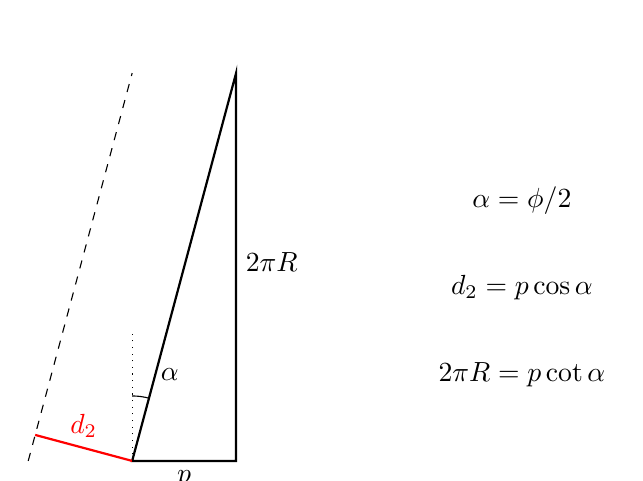
\begin{tikzpicture}[scale=1.1]
\draw[thick](0,0)--(1.2,0)--(1.2,4.478)--cycle;
\node[below]at(.6,0){$p$};\node[right]at(1.2,2.3){$2\pi R$};
\draw[dashed](-1.2,0)--(0,4.478);
\draw[red,thick](0,0)--(-1.1196,.3)node[midway,above]{$d_2$};
\draw[dotted](0,0)--(0,1.5);
\draw (0,.75)arc(90:75:.75);\node[right]at(.22,1){$\alpha$};
\node at(4.5,3){$\alpha=\phi/2$};\node at(4.5,2){$d_2=p\cos\alpha$};
\node at(4.5,1){$2\pi R=p\cot\alpha$};
\end{tikzpicture}
}
\ifdim\wd\diagrambox>.88\linewidth
\sbox{\diagrambox}{\resizebox{.88\linewidth}{!}{\usebox{\diagrambox}}}\fi
\ifdim\ht\diagrambox>.38\textheight
\resizebox{!}{.38\textheight}{\usebox{\diagrambox}}
\else\usebox{\diagrambox}\fi
\par\smallskip{\small 螺旋展开为直角三角形及法向间距\par}\endgroup\end{minipage}\end{center}

设展开螺旋线与圆周方向的夹角为
\(\alpha=\phi/2\)。相邻展开直线的轴向间隔是 \(p\)，法向间距为

\[
d_2=p\cos\alpha.
\]

因此

\[
\boxed{p=\frac{d_2}{\cos\alpha}
=\frac{\lambda L}{X_2\cos(\phi/2)}}.
\]

直角三角形还给出

\[
\tan\alpha=\frac{p}{2\pi R},
\]

所以

\[
\boxed{R=\frac{p}{2\pi\tan\alpha}
=\frac{\lambda L}{2\pi X_2\sin(\phi/2)}}.
\]

取 \(\phi=30^\circ\)，

\[
p=1.6191\,\mathrm{mm},\qquad R=0.9617\,\mathrm{mm}.
\]

按估算精度可写为

\[
\boxed{p\simeq1.6\,\mathrm{mm},\quad R\simeq0.96\,\mathrm{mm}}.
\]

\subsubsection{6.
DNA照片的阶次与尺度}\label{dnaux7167ux7247ux7684ux9636ux6b21ux4e0eux5c3aux5ea6}

图b中央零级不可见，第4级也缺失。可用第2、3、5级拟合周期，而不是把每一对可见斑点都视为相邻阶次。例如从第2级到第5级的距离应除以3。

对应法向条纹周期取 \(X'=4.7\,\mathrm{mm}\)，则

\[
d'=\frac{\lambda'L'}{X'}
=\frac{0.15\times10^{-9}\times0.090}
{4.7\times10^{-3}}\,\mathrm m
=2.87234\,\mathrm{nm}.
\]

此处 \(\lambda'\) 用纳米，而屏距和条纹间距统一用米；单位不能直接把
\(0.15\times9.0/4.7\) 当成纳米结果。

\subsubsection{7.
DNA半径和螺距}\label{dnaux534aux5f84ux548cux87baux8ddd}

取 \(\alpha'=\phi'/2=42^\circ\)，同样得到

\[
\boxed{p'=\frac{\lambda'L'}{X'\cos\alpha'}},
\qquad
\boxed{R'=\frac{\lambda'L'}{2\pi X'\sin\alpha'}}.
\]

数值为

\[
p'=3.8651\,\mathrm{nm},\qquad R'=0.6832\,\mathrm{nm}.
\]

依题设模型与照片读数，

\[
\boxed{p'\simeq3.9\,\mathrm{nm},\quad R'\simeq0.68\,\mathrm{nm}}.
\]

这里的结果应与题设的几何反演模型一起理解。题目不给完整原子散射因子或三维倒易空间资料，所以不能把本题估计值宣称为不受模型影响的精确分子结构测定。

\subsubsection{8.
小角度近似误差}\label{ux5c0fux89d2ux5ea6ux8fd1ux4f3cux8befux5dee}

若 \(X\) 是屏上坐标，从几何上
\(\sin\vartheta=X/\sqrt{L^2+X^2}\)。用于一级暗纹的精确尺度关系为

\[
d=\frac{\lambda\sqrt{L^2+X^2}}X.
\]

相对于 \(\lambda L/X\)，修正因子为

\[
\sqrt{1+(X/L)^2}\simeq1+\frac12(X/L)^2.
\]

对弹簧 \(X_1/L\simeq0.00188\)，修正远小于照片读数误差。对DNA
\(X'/L'\simeq0.0522\)，修正约0.14\%，仍小于约10\%的允许测量误差。

若使用较高阶纹，角度随阶次增加，应逐一检查
\(X_n/L\)；不能仅由第一阶的小角度保证整张照片都可使用同样精度。

\subsubsection{9. 误差传播}\label{ux8befux5deeux4f20ux64ad}

把 \(\alpha\) 以弧度表示，保持 \(\lambda,L\) 已知，有

\[
\frac{\delta d_1}{d_1}\simeq-\frac{\delta X_1}{X_1},
\]

\[
\frac{\delta p}{p}\simeq
-\frac{\delta X_2}{X_2}+\tan\alpha\,\delta\alpha,
\]

\[
\frac{\delta R}{R}\simeq
-\frac{\delta X_2}{X_2}-\cot\alpha\,\delta\alpha.
\]

因此弹簧 \(\alpha=15^\circ\)
时，半径对夹角误差比较敏感，而螺距较不敏感。若 \(\phi\) 误差为
\(2^\circ\)，则
\(\delta\alpha=1^\circ=0.01745\)，半径的角度误差贡献约为6.5\%。

DNA \(\alpha'=42^\circ\)
的正切和余切都接近1，半径和螺距对角度误差的敏感程度较接近。报很多有效数字并不能消除取点和照片模糊带来的误差。

\subsubsection{10.
结果的联合检查}\label{ux7ed3ux679cux7684ux8054ux5408ux68c0ux67e5}

四个尺度都必须为正，弹簧需满足
\(d_1\ll2R\)，且线圈之间有空间。由结果反算

\[
\frac{p}{2\pi R}=\tan15^\circ,
\qquad
\frac{p'}{2\pi R'}=\tan42^\circ,
\]

应恢复照片夹角。把 \(d_1,d_2\) 反代回
\(\lambda L/d\)，应分别恢复长周期和短周期。

这两类反算检验不同部分：前者检查螺旋展开几何，后者检查衍射尺度及单位换算。只与参考答案数字相近，并不能替代这些物理一致性检查。

\clearpage

\section{第 8 题
核反冲、共振窗口与微小频移测量（40分）}\label{ux7b2c-8-ux9898-ux6838ux53cdux51b2ux5171ux632fux7a97ux53e3ux4e0eux5faeux5c0fux9891ux79fbux6d4bux91cf40ux5206}

原子核能级间可通过吸收或发射光子跃迁。自由原子核吸收或发射光子时会反冲，部分能量转为原子核动能。激发态相对基态的能量不是完全确定的，而在以
\(E_0\) 为中心、宽度为 \(2\Gamma\) 的范围内取值。

对 \(\,{}^{57}\mathrm{Fe}\) 第一激发态到基态的跃迁，取

\[
E_0=2.31\times10^{-15}\,\mathrm J,\qquad
\Gamma\simeq3.2\times10^{-13}E_0,
\]

\[
m_{\rm Fe}\simeq9.5\times10^{-26}\,\mathrm{kg},
\quad h=6.6\times10^{-34}\,\mathrm{J\,s},
\quad c=3.0\times10^8\,\mathrm{m/s}.
\]

（1）忽略能级宽度，求发射的反冲能，并求考虑核反冲与不考虑核反冲时发射光子频率之差。

（2）忽略能级宽度，求吸收的反冲能，并求考虑核反冲与不考虑核反冲时吸收光子频率之差。

（3）考虑能级宽度，静止的激发态自由核发射的光子，能否被另一静止基态自由核共振吸收？说明理由。

（4）把核置于晶体中，按题设认为核跃迁无反冲。静止晶体中的激发核发射光子，另一以速度
\(V\)
运动的晶体中的基态核吸收。什么速度范围会共振？若到达吸收晶体的光子发生相对量级
\(10^{-10}\) 的微小频率变化，怎样测量？给出原理和计算。

\subsection{一、题型定位}\label{ux4e00ux9898ux578bux5b9aux4f4d-7}

本题比较反冲能、能级宽度和多普勒频移三个尺度。发射需要让部分跃迁能量成为核动能，光子能量偏低；吸收则同时需要提供激发能和反冲动能，光子能量偏高。

晶体无反冲时，两窗口中心恢复一致；人为调节晶体速度可使入射频率在吸收体参考系中移动，以补偿未知频移。测量时扫描速度并寻找吸收峰，再由峰位换算频移，便可避开直接测量光频微小差值的困难。

\subsection{二、知识点}\label{ux4e8cux77e5ux8bc6ux70b9-7}

光子的能量和动量满足

\[
E_\gamma=h\nu,\qquad p_\gamma=\frac{E_\gamma}{c}.
\]

核反冲在本题为非相对论运动，其动能为

\[
E_R=\frac{p_\gamma^2}{2m_{\rm Fe}}
=\frac{E_\gamma^2}{2m_{\rm Fe}c^2}.
\]

因为 \(E_0/(m_{\rm Fe}c^2)\ll1\)，可在反冲项中用
\(E_\gamma\simeq E_0\)，只保留反冲的一阶修正。

题给宽度 \(2\Gamma\) 是能量窗口总宽度，因此半宽为 \(\Gamma\)，频率半宽为
\(\Gamma/h\)。两窗口相交时允许共振，这里使用题设的有限窗口模型。

\subsection{三、物理图像}\label{ux4e09ux7269ux7406ux56feux50cf-7}

\begin{center}
\begin{minipage}{\linewidth}
\centering\begingroup\sbox{\diagrambox}{\small
\begin{tikzpicture}[scale=.9]
\node[left]at(0,2.55){发射};\fill[blue](1,1.8)circle(4pt);
\draw[arr,red](1.4,1.8)--(4.2,1.8)node[midway,above]{$E_\gamma/c$};
\draw[arr,blue](.7,1.8)--(-1.2,1.8)node[midway,below]{$p_{\rm recoil}$};
\node[left]at(0,.55){吸收};\draw[arr,red](-2,-.2)--(.6,-.2)node[midway,above]{$E_\gamma/c$};
\fill[blue](1,-.2)circle(4pt);\draw[arr,blue](1.4,-.2)--(3.7,-.2)node[midway,below]{$p_{\rm recoil}$};
\node at(2,-1.1){发射少$E_R$；吸收多$E_R$};
\end{tikzpicture}
}
\ifdim\wd\diagrambox>.88\linewidth
\sbox{\diagrambox}{\resizebox{.88\linewidth}{!}{\usebox{\diagrambox}}}\fi
\ifdim\ht\diagrambox>.38\textheight
\resizebox{!}{.38\textheight}{\usebox{\diagrambox}}
\else\usebox{\diagrambox}\fi
\par\smallskip{\small 自由核发射与吸收时的动量及能量分配\par}\endgroup\end{minipage}\end{center}

发射时光子与核动量相反；吸收时初始光子动量成为核的反冲动量。两过程反冲动能都是正的，但在光子能量方程中位于不同侧。

\begin{center}
\begin{minipage}{\linewidth}
\centering\begingroup\sbox{\diagrambox}{\small
\begin{tikzpicture}[xscale=1.1]
\draw[arr](0,0)--(8,0)node[right]{$E$};
\draw[very thick,blue](1.3,.5)--(2.1,.5); \draw[very thick,red](5.3,.5)--(6.1,.5);
\draw[dashed](1.7,0)--(1.7,1.1)node[above]{$E_0-E_R$};
\draw[dashed](5.7,0)--(5.7,1.1)node[above]{$E_0+E_R$};
\draw[<->](1.7,-.6)--(5.7,-.6)node[midway,below]{$2E_R\gg2\Gamma$};
\node at(4,1.8){图中窗口宽度放大，真实尺度差约$4.2\times10^5$};
\end{tikzpicture}
}
\ifdim\wd\diagrambox>.88\linewidth
\sbox{\diagrambox}{\resizebox{.88\linewidth}{!}{\usebox{\diagrambox}}}\fi
\ifdim\ht\diagrambox>.38\textheight
\resizebox{!}{.38\textheight}{\usebox{\diagrambox}}
\else\usebox{\diagrambox}\fi
\par\smallskip{\small 自由核的发射和吸收窗口相隔两份反冲能\par}\endgroup\end{minipage}\end{center}

两窗口中心分别为 \(E_0-E_R\) 和 \(E_0+E_R\)，间隔为
\(2E_R\)。不能只拿单个窗口半宽与两个中心之间的距离比较，却忘记吸收窗口也有半宽。

无反冲晶体的窗口都以 \(E_0\)
为中心。只要晶体相对光子传播方向有速度分量，多普勒效应就把入射窗口相对吸收窗口移动。

\subsection{四、解题入口}\label{ux56dbux89e3ux9898ux5165ux53e3-7}

先用动量守恒求反冲速度与动能，再分别列发射、吸收能量式。把 \(E_R\) 与
\(\Gamma\) 的比值算出来，第三问的答案立即明确。

第四问先约定速度符号。以下以吸收晶体沿光子传播方向运动为
\(u>0\)，即远离光源；迎着光子运动为 \(u<0\)。\(V=|u|\)
是速度大小。这个约定能让补偿未知频移时的方向一目了然。

比较窗口交叠时，可先用
\(\nu'\simeq\nu(1-u/c)\)，再给出精确纵向多普勒结果作为检查。原题数值只需一阶近似。

\subsection{五、解析}\label{ux4e94ux89e3ux6790-7}

\subsubsection{1.
共同的反冲尺度}\label{ux5171ux540cux7684ux53cdux51b2ux5c3aux5ea6}

不计反冲时，

\[
\nu_0=\frac{E_0}{h}
=3.50\times10^{18}\,\mathrm{Hz}.
\]

光子动量近似为

\[
p_0=\frac{E_0}{c}=7.70\times10^{-24}\,\mathrm{kg\,m/s}.
\]

核反冲速度为

\[
v_R\simeq\frac{E_0}{m_{\rm Fe}c}
=81.05\,\mathrm{m/s}\ll c.
\]

故采用非相对论核动能合理。反冲能为

\[
\boxed{E_R\simeq\frac{E_0^2}{2m_{\rm Fe}c^2}
=3.1205\times10^{-22}\,\mathrm J}.
\]

它相对跃迁能很小，但是否可以忽略还要与能级宽度比较，不能仅凭
\(E_R/E_0\ll1\) 下结论。

\subsubsection{2.
发射光子的频率}\label{ux53d1ux5c04ux5149ux5b50ux7684ux9891ux7387}

初始激发核静止，发射后光子与核反冲动量大小相等。能量守恒为

\[
E_0=h\nu_{\rm em}
+\frac{(h\nu_{\rm em})^2}{2m_{\rm Fe}c^2}.
\]

在反冲项中用 \(h\nu_{\rm em}\simeq E_0\)，

\[
h\nu_{\rm em}\simeq E_0-E_R.
\]

所以

\[
\boxed{\nu_{\rm em}-\nu_0\simeq-\frac{E_R}{h}
=-4.7281\times10^{11}\,\mathrm{Hz}}.
\]

负号表示发射光子频率比不反冲时低。核动能来自原来的跃迁能，不能把反冲能加到发射光子上。

\subsubsection{3.
吸收光子的频率}\label{ux5438ux6536ux5149ux5b50ux7684ux9891ux7387}

初始基态核静止，吸收后既被激发，又获得光子动量。能量守恒为

\[
h\nu_{\rm abs}=E_0
+\frac{(h\nu_{\rm abs})^2}{2m_{\rm Fe}c^2}.
\]

一阶近似给出

\[
h\nu_{\rm abs}\simeq E_0+E_R,
\]

于是

\[
\boxed{\nu_{\rm abs}-\nu_0\simeq+\frac{E_R}{h}
=+4.7281\times10^{11}\,\mathrm{Hz}}.
\]

吸收需要比跃迁能更多的光子能量，额外能量提供核的反冲动能。两过程的反冲能在一阶精度下相等，符号差别属于光子能量而不是动能。

\subsubsection{4.
近似精度与稳定求根}\label{ux8fd1ux4f3cux7cbeux5ea6ux4e0eux7a33ux5b9aux6c42ux6839}

令

\[
\epsilon=\frac{E_0}{m_{\rm Fe}c^2}
\simeq2.70\times10^{-7}.
\]

反冲能相对修正为
\(\epsilon/2\)。在非相对论模型内，两个能量方程的小根可以写成稳定形式

\[
E_{\rm em}=
\frac{2E_0}{1+\sqrt{1+2\epsilon}},
\]

\[
E_{\rm abs}=
\frac{2E_0}{1+\sqrt{1-2\epsilon}}.
\]

展开后分别恢复
\(E_0\mp E_R\)。稳定形式避免直接相减两个几乎相等的大数造成数值精度损失。

这些平方根式是非相对论反冲模型的自洽求根，不是全相对论精确核跃迁式。本题已足以用一阶反冲分析；把修正差异视为模型精度，不应赋予多余有效数字。

\subsubsection{5.
自由核的窗口是否相交}\label{ux81eaux7531ux6838ux7684ux7a97ux53e3ux662fux5426ux76f8ux4ea4}

能级窗口为 \(E_0-\Gamma\) 到
\(E_0+\Gamma\)。在一阶反冲近似中，发射和吸收窗口分别近似为

\[
\mathcal I_{\rm em}=
[E_0-E_R-\Gamma,\ E_0-E_R+\Gamma],
\]

\[
\mathcal I_{\rm abs}=
[E_0+E_R-\Gamma,\ E_0+E_R+\Gamma].
\]

窗口相交要求发射的最高能量不低于吸收的最低能量：

\[
E_0-E_R+\Gamma\ge E_0+E_R-\Gamma.
\]

即

\[
\boxed{E_R\le\Gamma}.
\]

等号只有窗口端点接触，是阈值情形；实际有宽度的重叠需要严格小于。现在

\[
\Gamma=7.392\times10^{-28}\,\mathrm J,
\qquad
\frac{E_R}{\Gamma}\simeq4.22\times10^5.
\]

因此按题设有限能量窗口模型，两个静止自由核不能共振吸收。虽然 \(E_R\) 比
\(E_0\) 小约七个数量级，却比 \(\Gamma\) 大五个数量级。

\subsubsection{6.
晶体无反冲后的窗口}\label{ux6676ux4f53ux65e0ux53cdux51b2ux540eux7684ux7a97ux53e3}

按题设，核置于晶体时跃迁不产生可观测反冲损失。发射和吸收的能量窗口均为

\[
\mathcal I_0=[E_0-\Gamma,E_0+\Gamma].
\]

不需把晶体中的单核仍当作自由核来使用前面的
\(m_{\rm Fe}\)。这里采用的是题目指定的无反冲条件；更完整的晶体模型会涉及晶格及声子，原题不要求计算这些效应。

吸收晶体以 \(u>0\) 沿光子方向运动时，看到的纵向多普勒因子为

\[
D_u=\sqrt{\frac{1-\beta}{1+\beta}},
\qquad\beta=\frac uc.
\]

小速度下
\(D_u\simeq1-u/c\)，所以远离光源使入射频率降低，迎向光源使频率升高。

\subsubsection{7.
共振速度范围}\label{ux5171ux632fux901fux5ea6ux8303ux56f4}

运动后的入射窗口为

\[
D_u[E_0-\Gamma,E_0+\Gamma].
\]

与吸收体自身窗口相交，要求

\[
\frac{E_0-\Gamma}{E_0+\Gamma}
\le D_u\le
\frac{E_0+\Gamma}{E_0-\Gamma}.
\]

用精确多普勒因子求出对称界限，

\[
|\beta|\le
\frac{2E_0\Gamma}{E_0^2+\Gamma^2}.
\]

因 \(\Gamma/E_0\ll1\)，

\[
\boxed{|u|\lesssim\frac{2\Gamma}{E_0}c
=1.92\times10^{-4}\,\mathrm{m/s}
=0.192\,\mathrm{mm/s}}.
\]

所以沿光线方向运动时，速度大小应满足
\(0\le V\lesssim0.19\,\mathrm{mm/s}\)。若晶体运动方向并不沿光线，低速时应限制其沿光线的速度分量，不能只凭总速率判断一阶频移。

这里出现系数2，是因为发射窗口与吸收窗口各有半宽
\(\Gamma\)，允许的窗口中心相对偏移约为 \(2\Gamma\)。

\subsubsection{8.
用速度补偿测量微小频移}\label{ux7528ux901fux5ea6ux8865ux507fux6d4bux91cfux5faeux5c0fux9891ux79fb}

设入射光子在到达吸收体前发生未知相对频移

\[
\delta=\frac{\nu_{\rm in}-\nu_0}{\nu_0},
\qquad |\delta|\sim10^{-10}.
\]

改变吸收晶体沿光线的速度，测量吸收强度。吸收峰中心出现在

\[
\nu_{\rm in}D_u=\nu_0.
\]

一阶展开，

\[
(1+\delta)(1-u/c)\simeq1,
\]

所以

\[
\boxed{u_*\simeq c\delta}.
\]

若频率升高
\(\delta=+10^{-10}\)，吸收体沿光线远离源，以红移补偿；若频率降低，则向源移动。所需速度量级为

\[
\boxed{|u_*|\simeq0.030\,\mathrm{m/s}=3.0\,\mathrm{cm/s}}.
\]

\begin{center}
\begin{minipage}{\linewidth}
\centering\begingroup\sbox{\diagrambox}{\small
\begin{tikzpicture}[xscale=1.1,yscale=2]
\draw[arr](-3.2,0)--(3.4,0)node[right]{$u$};
\draw[arr](-3.2,0)--(-3.2,1.3)node[above]{吸收强度};
\draw[blue,thick,domain=-3:3,samples=100]plot(\x,{1/(1+20*(\x-1)^2)});
\draw[dashed](1,0)--(1,1)node[above]{$u_* \simeq c\delta$};
\node at(-.7,.9){调节速度使频率补偿};
\end{tikzpicture}
}
\ifdim\wd\diagrambox>.88\linewidth
\sbox{\diagrambox}{\resizebox{.88\linewidth}{!}{\usebox{\diagrambox}}}\fi
\ifdim\ht\diagrambox>.38\textheight
\resizebox{!}{.38\textheight}{\usebox{\diagrambox}}
\else\usebox{\diagrambox}\fi
\par\smallskip{\small 扫描吸收体速度，由共振峰位置测量频移\par}\endgroup\end{minipage}\end{center}

\subsubsection{9.
为什么速度测量具有放大作用}\label{ux4e3aux4ec0ux4e48ux901fux5ea6ux6d4bux91cfux5177ux6709ux653eux5927ux4f5cux7528}

目标频移的绝对值约为

\[
|\Delta\nu|\sim\nu_0\times10^{-10}
=3.50\times10^8\,\mathrm{Hz}.
\]

尽管这个数不小，相对光频仍只有
\(10^{-10}\)。直接测光频差需要极高相对精度，速度补偿把它转化为容易控制的厘米每秒量级。

题给能级频率半宽为

\[
\Gamma/h=1.12\times10^6\,\mathrm{Hz},
\]

对应单个窗口半宽的速度尺度

\[
c\Gamma/E_0=0.096\,\mathrm{mm/s}.
\]

共振窗口重叠容许范围约为这个尺度的两倍。目标补偿速度比该范围大约156倍，扫描吸收峰可清楚区分``未补偿''和``已补偿''的状态。

\subsubsection{10.
精确补偿关系}\label{ux7cbeux786eux8865ux507fux5173ux7cfb}

若要保留纵向多普勒精确关系，令 \(\nu_{\rm in}=(1+\delta)\nu_0\)，则

\[
D_u=\frac1{1+\delta}.
\]

解得

\[
\boxed{\frac{u_*}{c}
=\frac{(1+\delta)^2-1}{(1+\delta)^2+1}}.
\]

展开首项为 \(u_*/c=\delta+O(\delta^2)\)。对 \(10^{-10}\)
的频移，一阶公式足够。正负号与前述速度约定一致。

实际测量可用未发生目标频移时的吸收峰作基准，再比较两次峰中心速度差，避免把装置固定的频率偏差混入目标变化。

\end{document}
